\section{Results}

{Our} algorithm is implemented in C++, {using} Eigen \cite{eigenweb} for the linear algebra routines, CGAL \cite{cgal2008computational} and Geogram \cite{levy2015geogram} for predicates and geometric kernel, libigl \cite{jacobson2016libigl} for basic geometry processing routines, and
meshio \cite{schlomer2020nschloe} for converting across the different formats.
We run our experiments on cluster nodes with Intel Xeon Platinum 8268 CPU 2.90GHz.
The reference implementation and the data used to generate the results will be released as an open-source project.


\begin{figure}
    \centering\small
    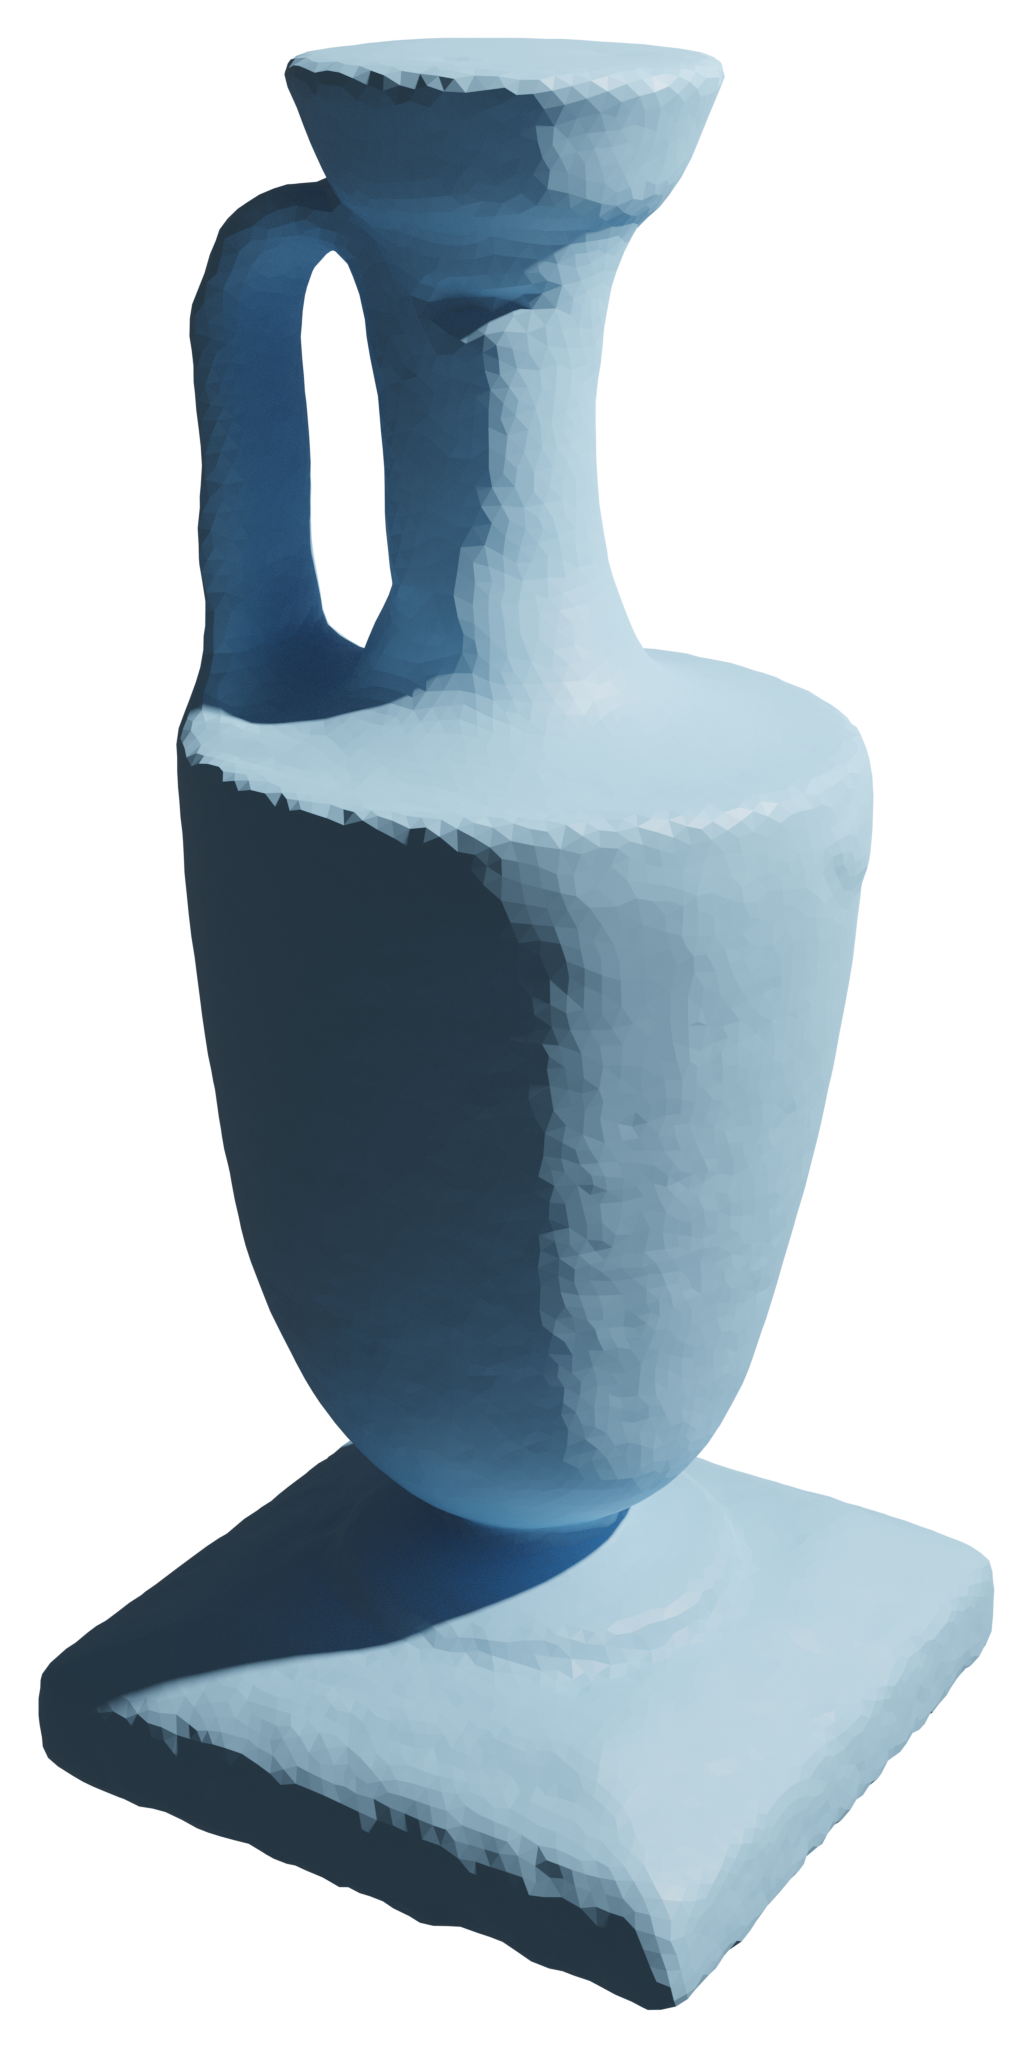
\includegraphics[width=.23\linewidth]{curve_meshing_in_shell_tex/figs/anphora/0005}
    \hfill
    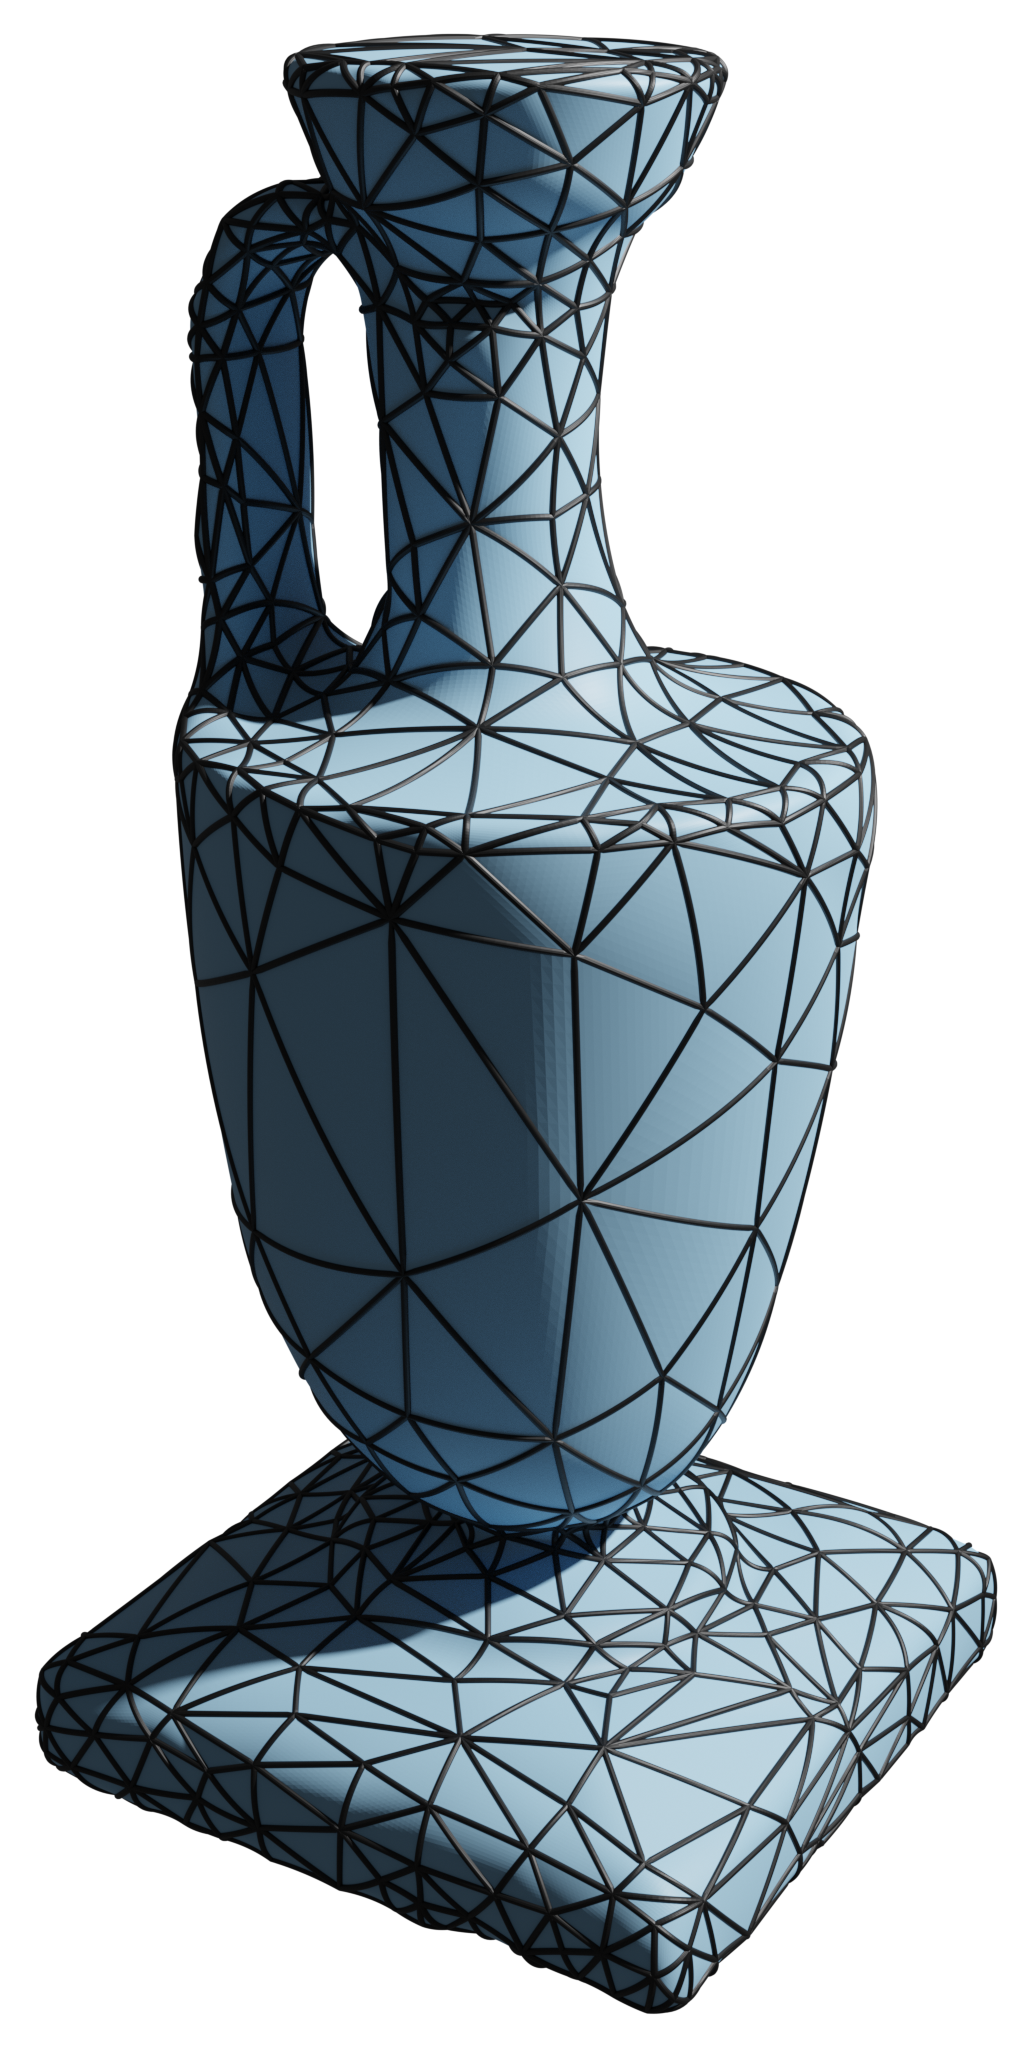
\includegraphics[width=.23\linewidth]{curve_meshing_in_shell_tex/figs/anphora/0001}\hfill
    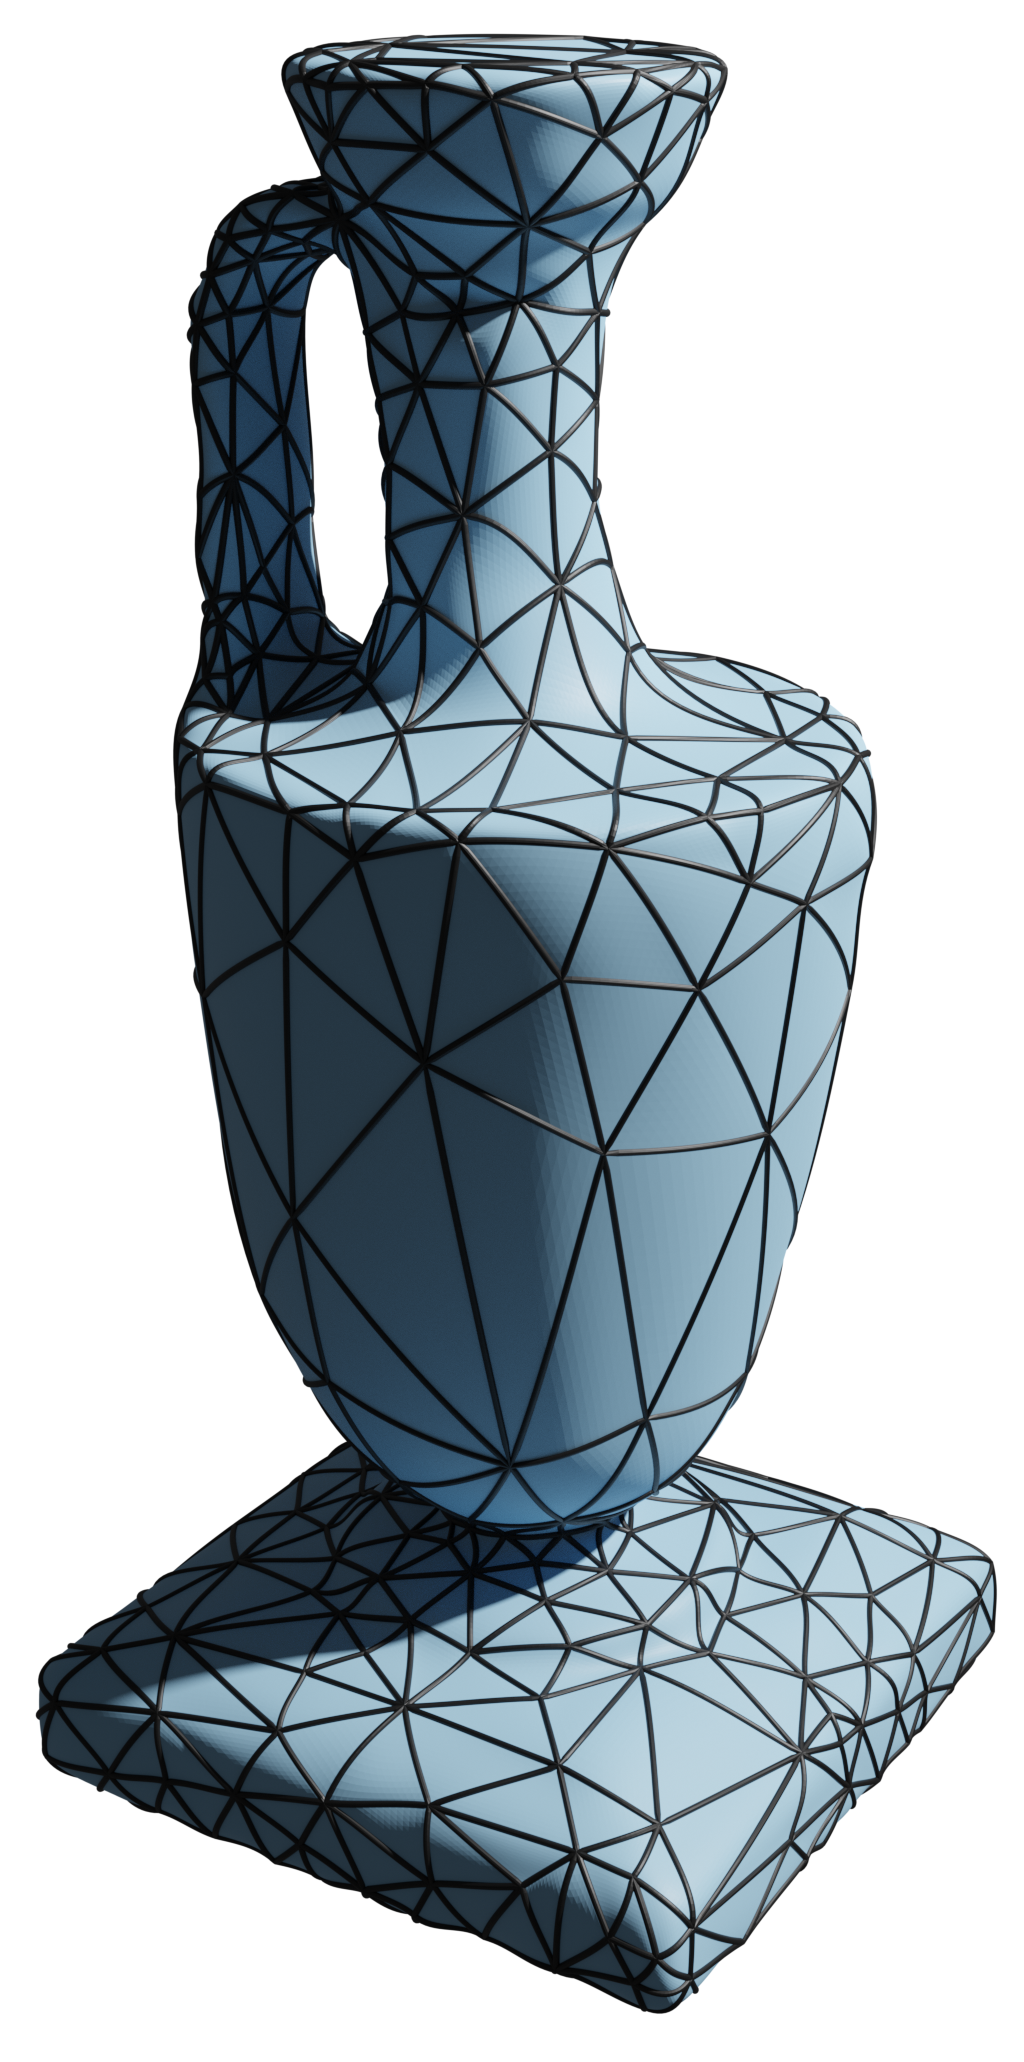
\includegraphics[width=.23\linewidth]{curve_meshing_in_shell_tex/figs/anphora/0002}\hfill
    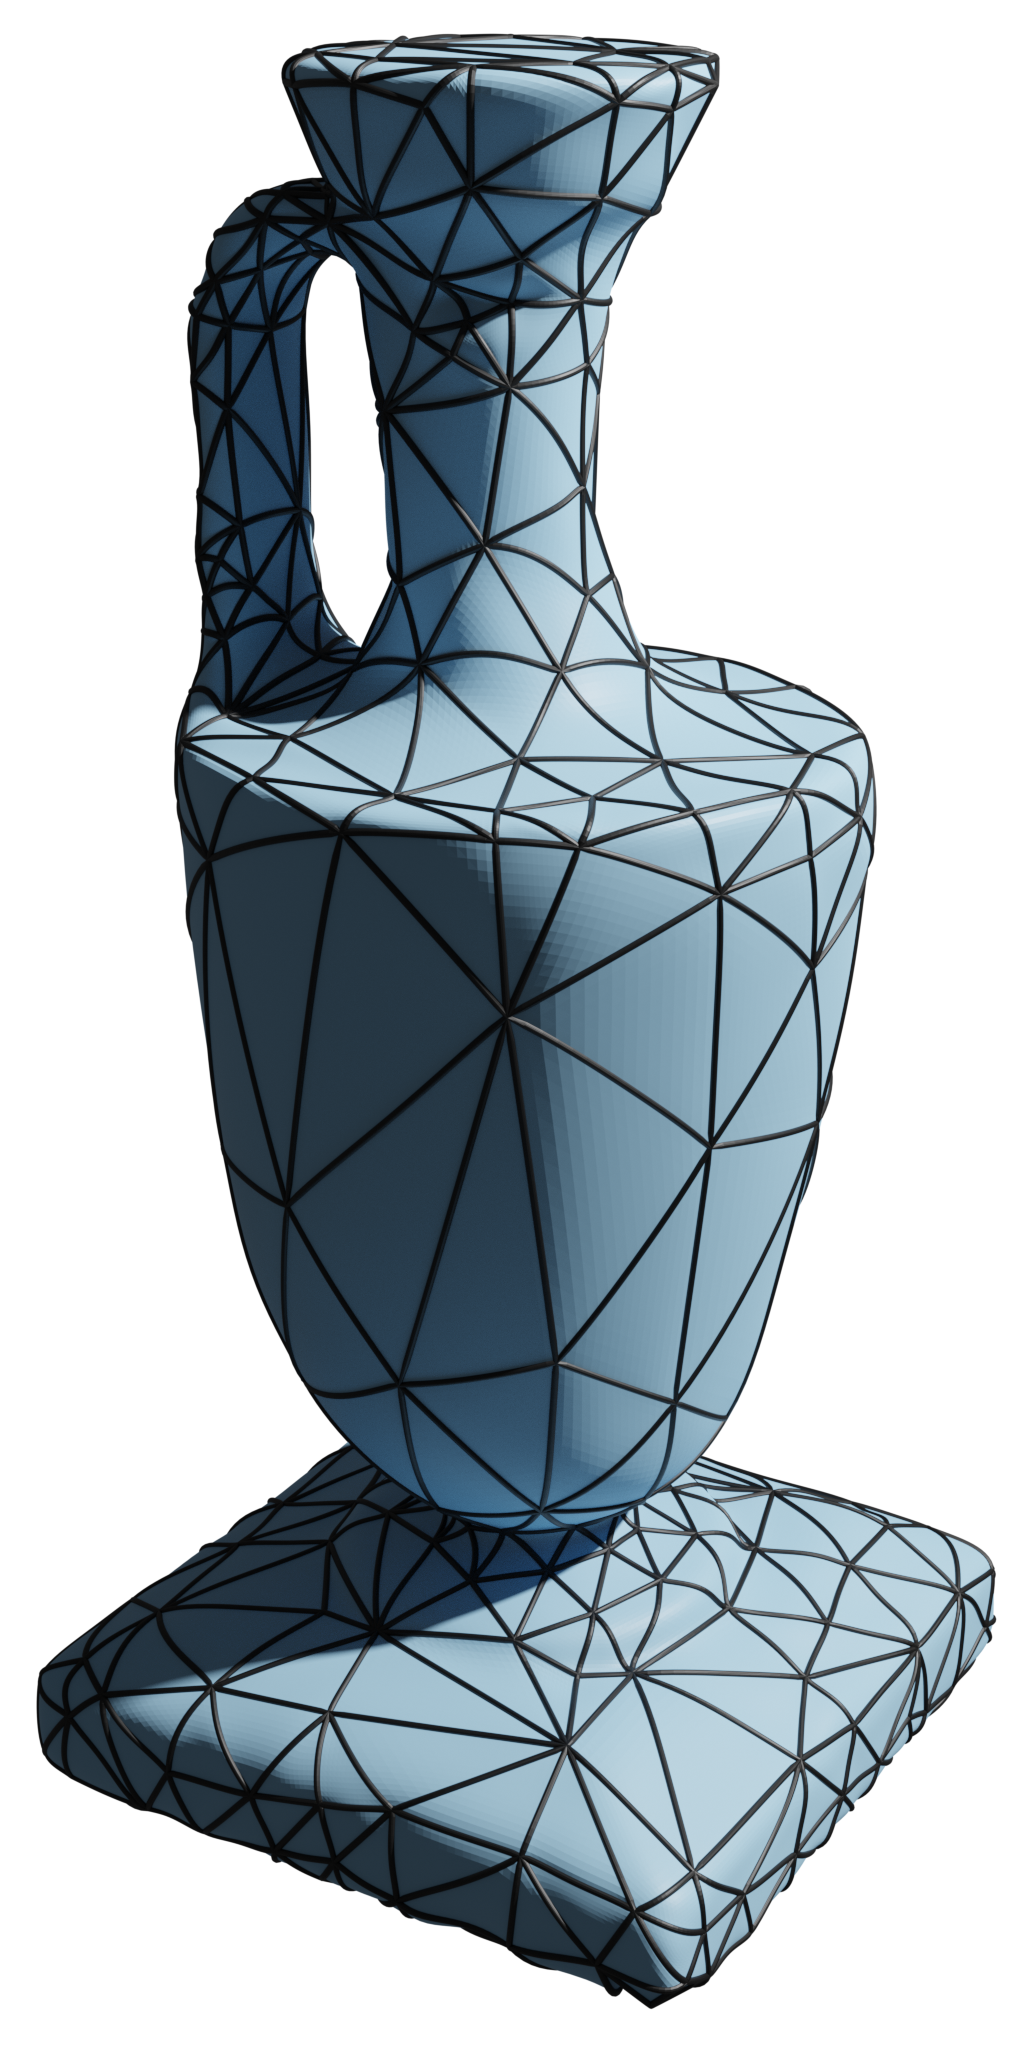
\includegraphics[width=.23\linewidth]{curve_meshing_in_shell_tex/figs/anphora/0003}
     \parbox{.24\linewidth}{\centering Input}\hfill
    \parbox{.24\linewidth}{\centering $k=3$}\hfill
    \parbox{.24\linewidth}{\centering $k=4$}\hfill
    \parbox{.24\linewidth}{\centering $k=5$}
    \caption{Curved meshes of different order. The additional degrees of freedom allows for more coarsening.}
    \label{bichon:fig:diff-k}
\end{figure}

To simplify the exposition, all meshes presented in this section are quartic meshes ($k=4$). Our method is flexible and, for lower $k$, it will generate denser meshes (Figure~\ref{bichon:fig:diff-k}).

\subsection{Large Scale Validation.}

We tested the robustness and quality of the result produced by our algorithm on three datasets: (1) Thingi10k dataset \cite{zhou2016thingi10k} containing 3574 models without features; (2) the first chunk {of} the ABC dataset~\cite{koch2019abc} with 5328 models with features marked from the STEP file and (3) the CAD dataset~\cite{Gao:2019} containing 106 models with semi-manual features.
%\ZJ{47 Thingi, 60 ABC out-of-time 12 hours}

Note that the original datasets contain more models since, for each of them, we selected meshes satisfying our assumptions: intersection-free (using the same strategy as in~\ref{chp:shell} with a distance tolerance of $10^{-6}$ and dihedral angle of $2^\circ$) oriented, manifold triangle meshes, smallest triangle area larger than $10^{-8}$. 





\begin{figure}
    \centering
    % \includegraphics{}
    \parbox{0.02\linewidth}{~}\hfill\hfill
    \parbox{.3\linewidth}{\centering Thingi10k}\hfill
    \parbox{.3\linewidth}{\centering ABC}\hfill
    \parbox{.3\linewidth}{\centering CAD}\par
    %
    \parbox{0.02\linewidth}{\centering\rotatebox{90}{\scriptsize{Edge length \%}}}\hfill\hfill
    \parbox{.3\linewidth}{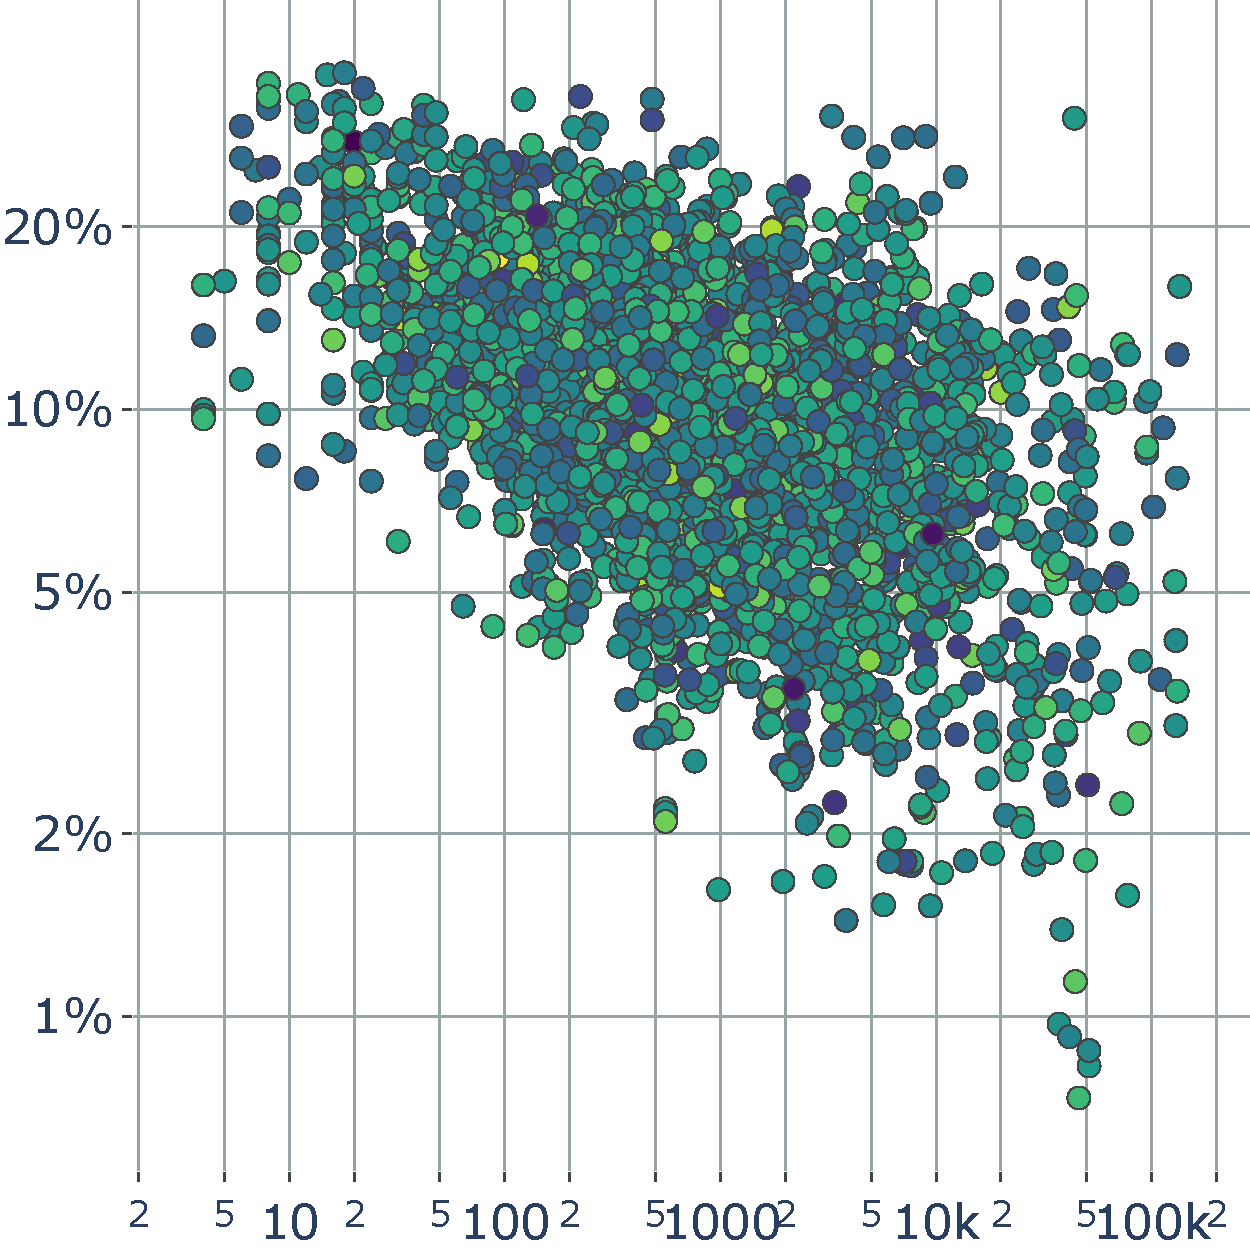
\includegraphics[width=\linewidth]{curve_meshing_in_shell_tex/figs/stats/edgelength_Thingi10k}}\hfill
    \parbox{.3\linewidth}{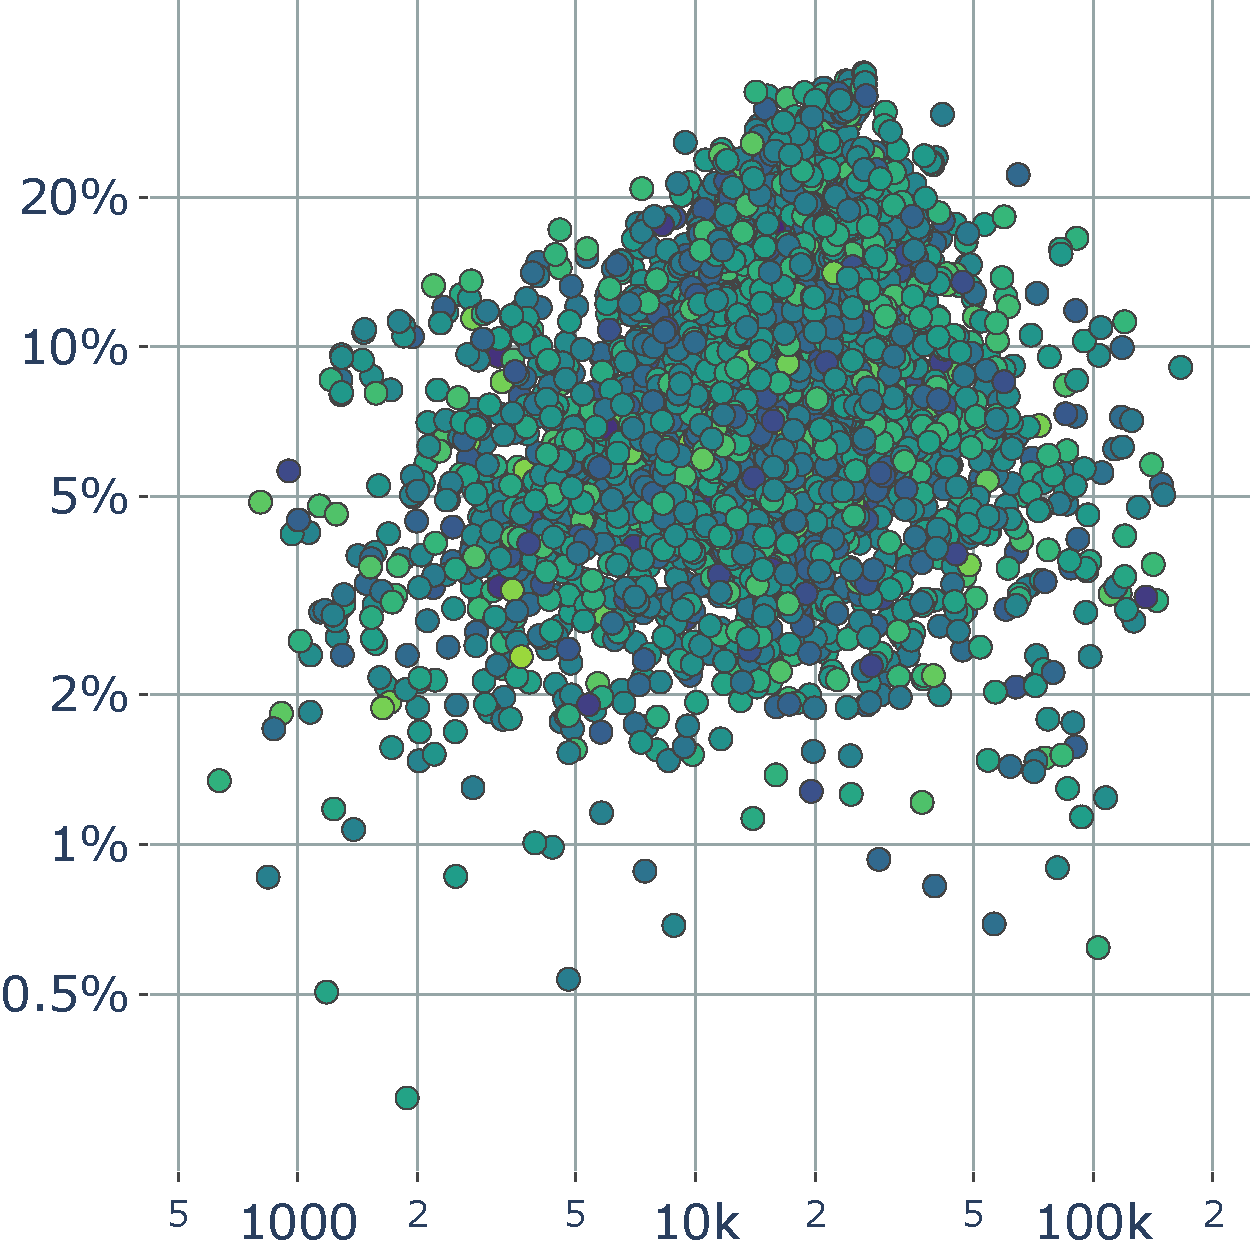
\includegraphics[width=\linewidth]{curve_meshing_in_shell_tex/figs/stats/edgelength_ABC}}\hfill
    \parbox{.3\linewidth}{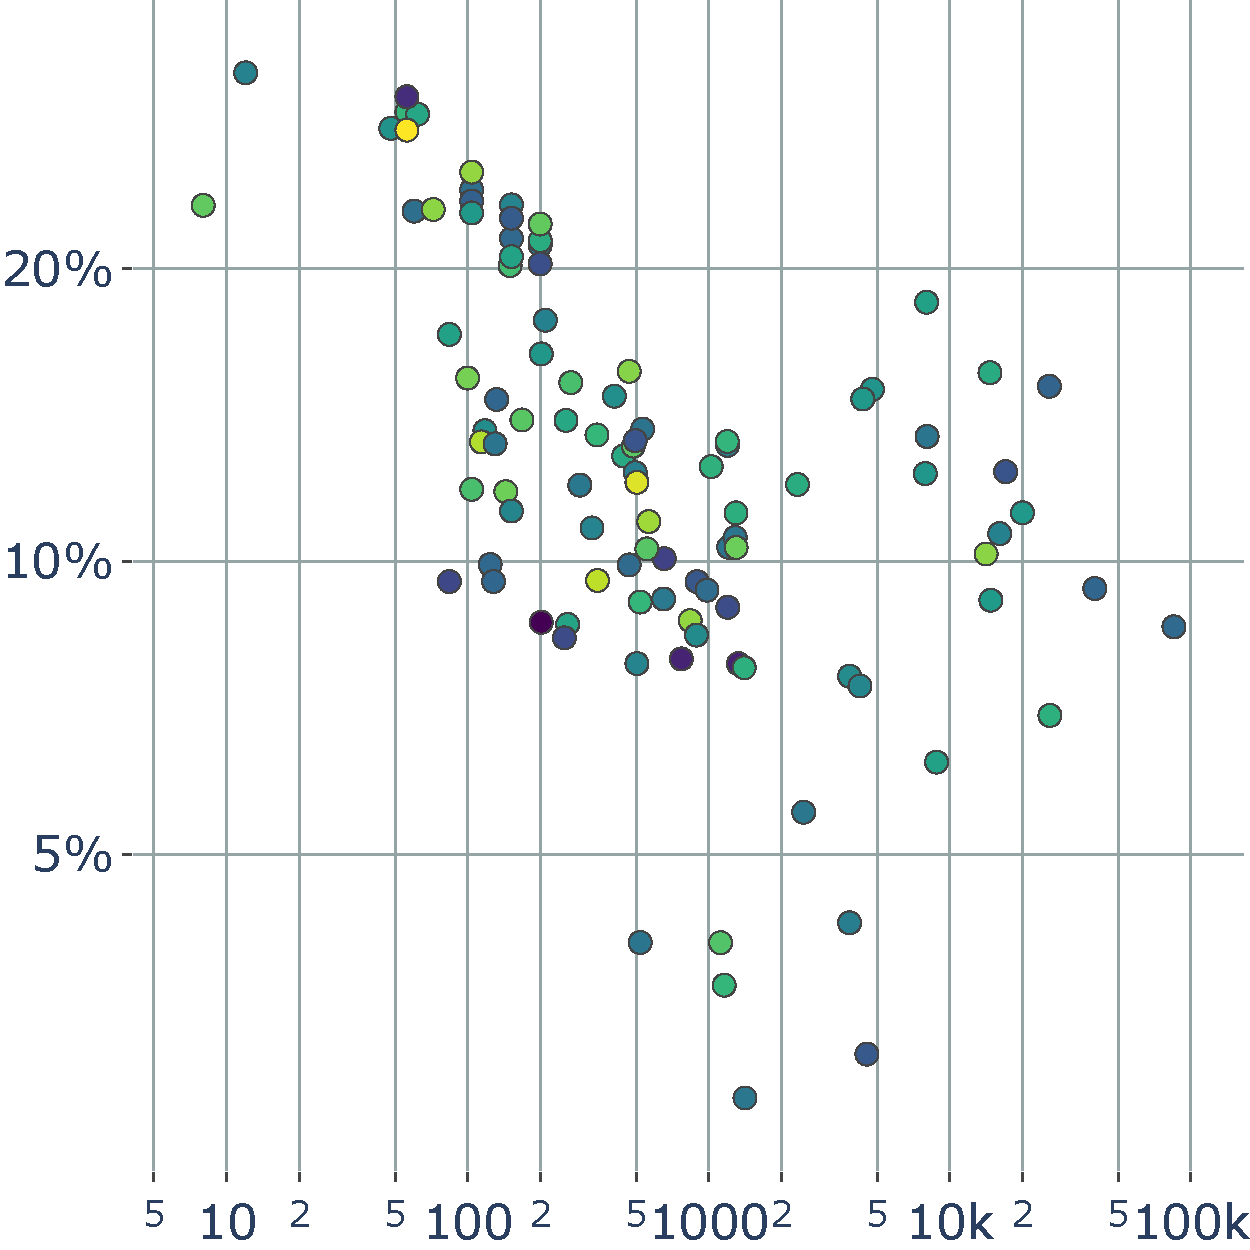
\includegraphics[width=\linewidth]{curve_meshing_in_shell_tex/figs/stats/edgelength_PolyCube}}\par
    \scriptsize{Input Vertices}
    \caption{Relative average edge length (with respect to longest bounding box edge of each model) of our curved meshes versus number of input vertices.}
    \label{bichon:fig:tet-count}
\end{figure}


\begin{figure}
    \centering\small
    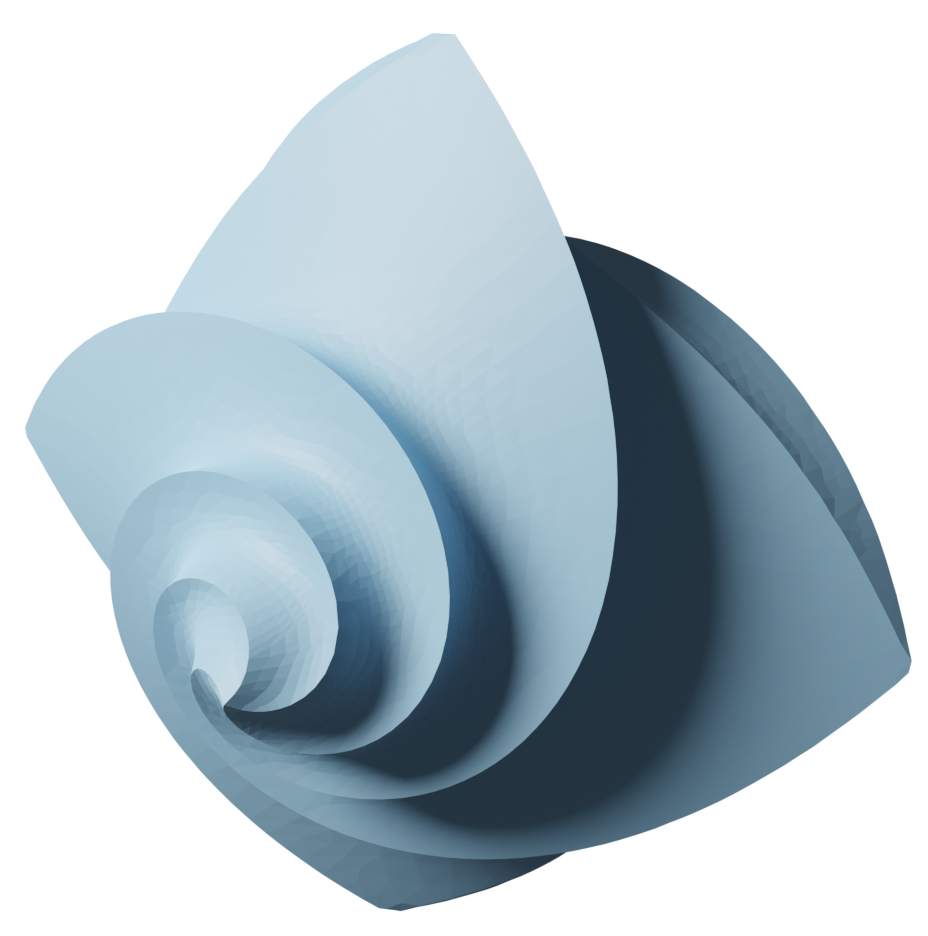
\includegraphics[width=.32\linewidth]{curve_meshing_in_shell_tex/figs/octa/0003}\hfill
    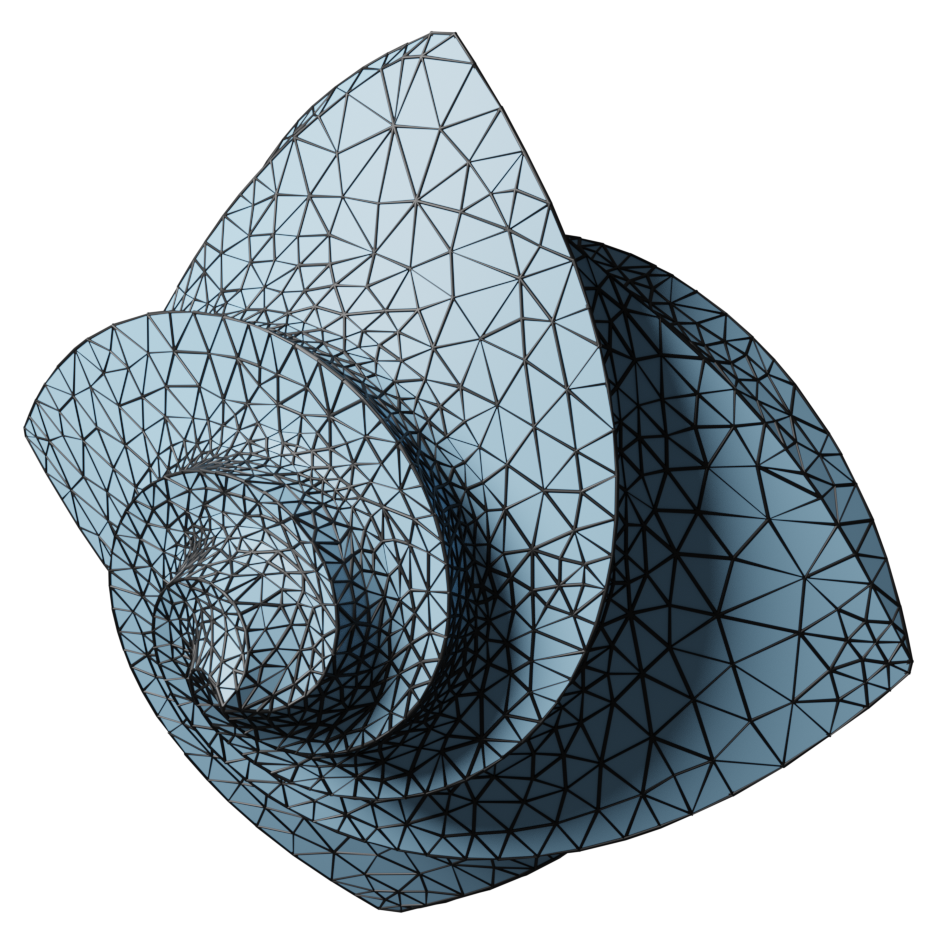
\includegraphics[width=.32\linewidth]{curve_meshing_in_shell_tex/figs/octa/0002}\hfill
    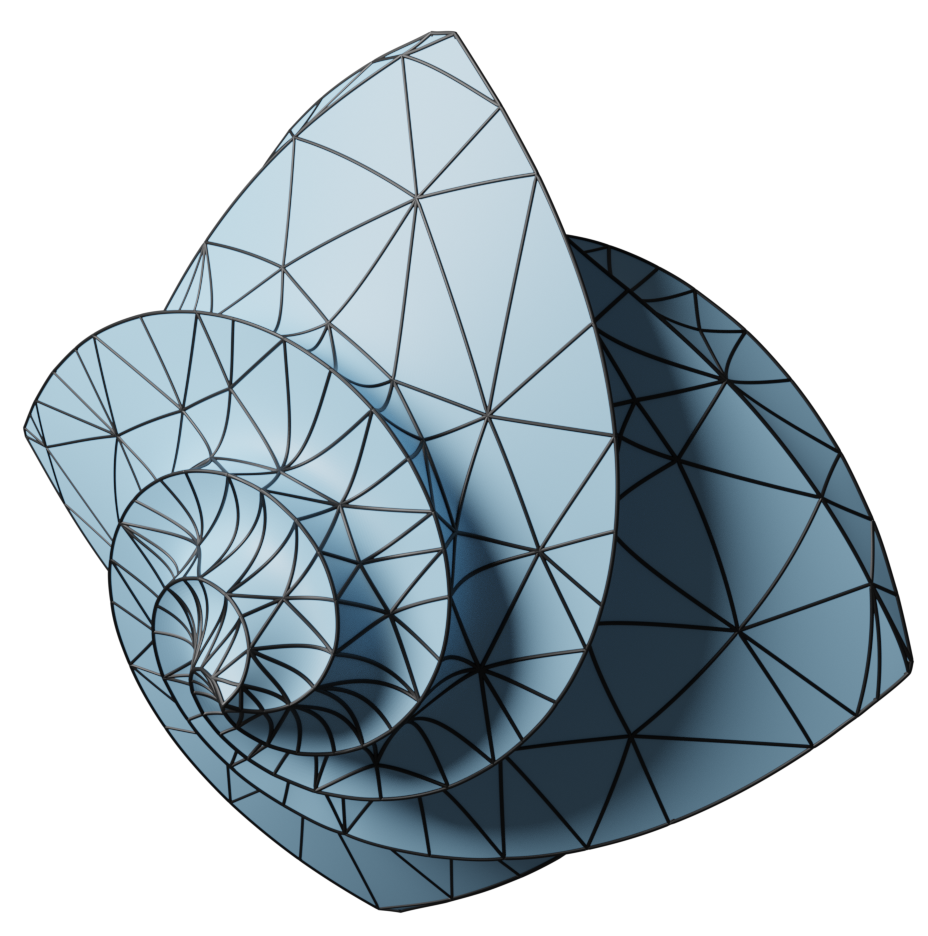
\includegraphics[width=.32\linewidth]{curve_meshing_in_shell_tex/figs/octa/0001}\par
    \parbox{.32\linewidth}{\centering Input}\hfill
    \parbox{.32\linewidth}{\centering fTetWild}\hfill
    \parbox{.32\linewidth}{\centering Ours}
    \caption{Within the same distance bound ($10^{-3}$ of the longest bounding box side), our method generates a coarser high order mesh, compared to the linear counterpart generated by fTetWild.}
    \label{bichon:fig:us-vs-ftetwild}
\end{figure}

Our method has only the geometry accuracy parameter $\varepsilon$, which we set to $1\%$ {of the longest bounding box edge}, and the point set $\P$ which we set {as} the input vertices $V$. 
With this basic setup, our algorithm aims to produce the coarsest possible mesh while preserving features and striving to generate high-quality meshes.
Our algorithm successfully generates curved meshes for 3527 for Thingi10k, 5268 for the ABC, and all for CAD dataset within 12 {hours}; by allowing more time, all models but 3 can be successfully processed. 
The 3 failures are due to models with a small one-tetrahedra component {that} ``move'' inside the shell as it grows. This is an implementation choice: we use collision detection instead of continuous collision detection for efficiency reasons.

Our method successfully {generates} coarse meshes whose average edge length is 10\% of the model size while preserving features (Figure~\ref{bichon:fig:tet-count}).
Figure~\ref{bichon:fig:us-vs-ftetwild} shows how our method successfully {captures} the features and coarsen the surface with curved elements, while many linear elements (generated with fTetWild~\cite{Hu:2020:fTetWild}) are required to closely approximate the surface.


\begin{figure}
    \centering
    % \includegraphics{}
    \parbox{0.02\linewidth}{~}\hfill\hfill
    \parbox{.3\linewidth}{\centering Thingi10k}\hfill
    \parbox{.3\linewidth}{\centering ABC}\hfill
    \parbox{.3\linewidth}{\centering CAD}\par
    %
    \parbox{0.02\linewidth}{\centering\rotatebox{90}{\scriptsize{Volume energy}}}\hfill\hfill
    \parbox{.3\linewidth}{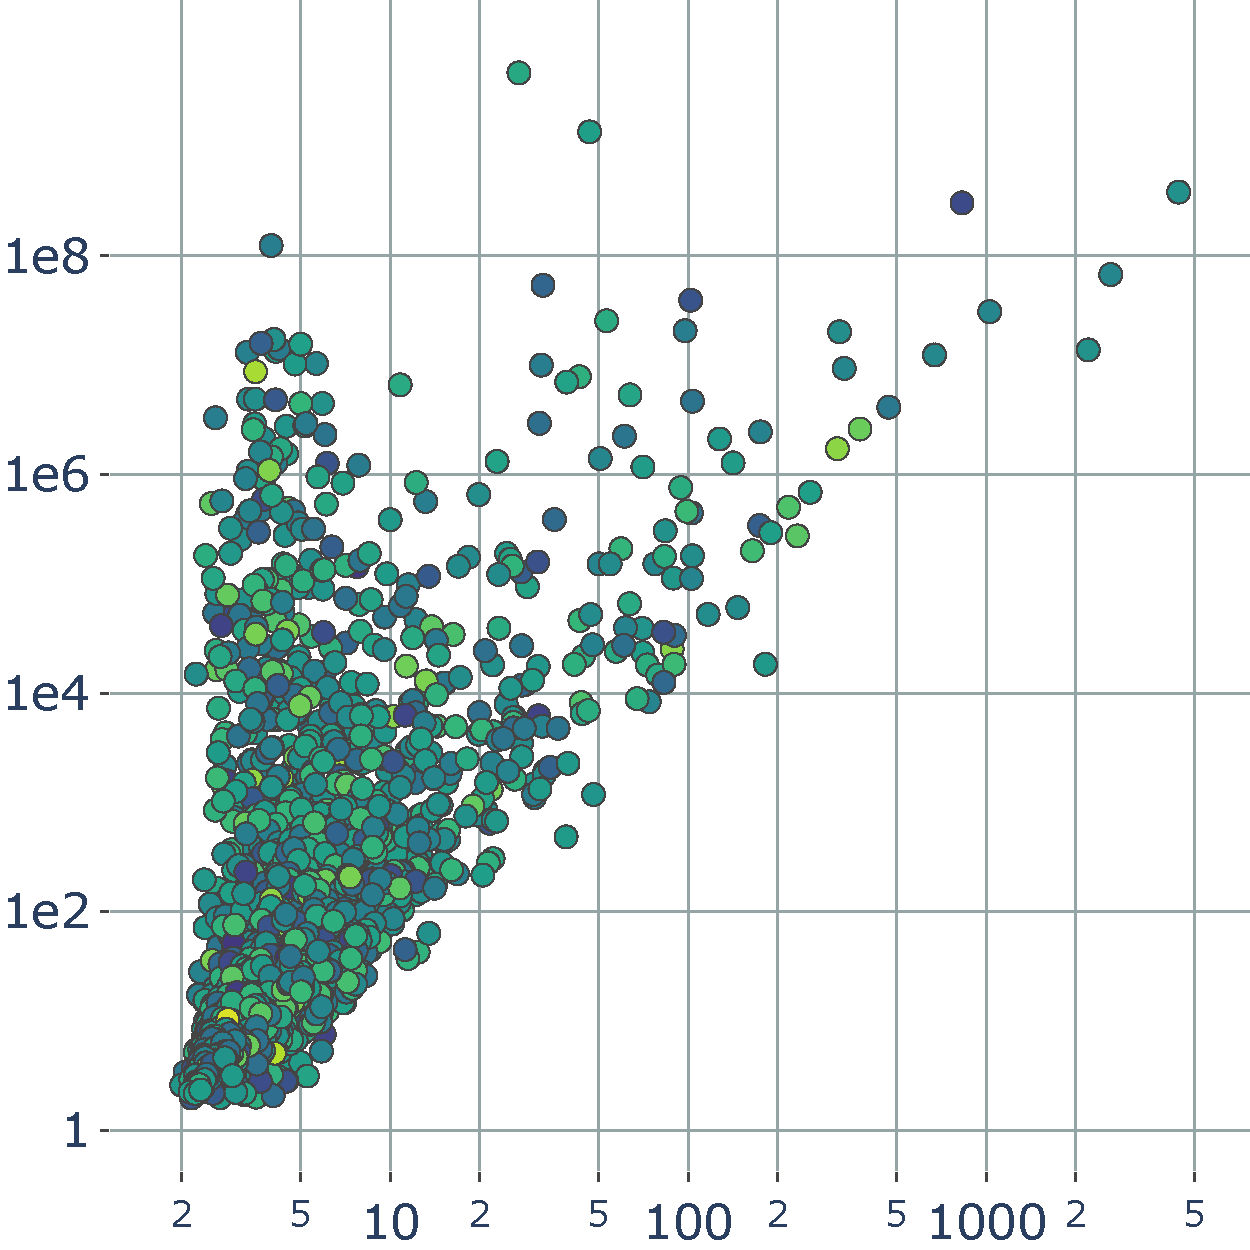
\includegraphics[width=\linewidth]{curve_meshing_in_shell_tex/figs/stats/energy_Thingi10k}}\hfill
    \parbox{.3\linewidth}{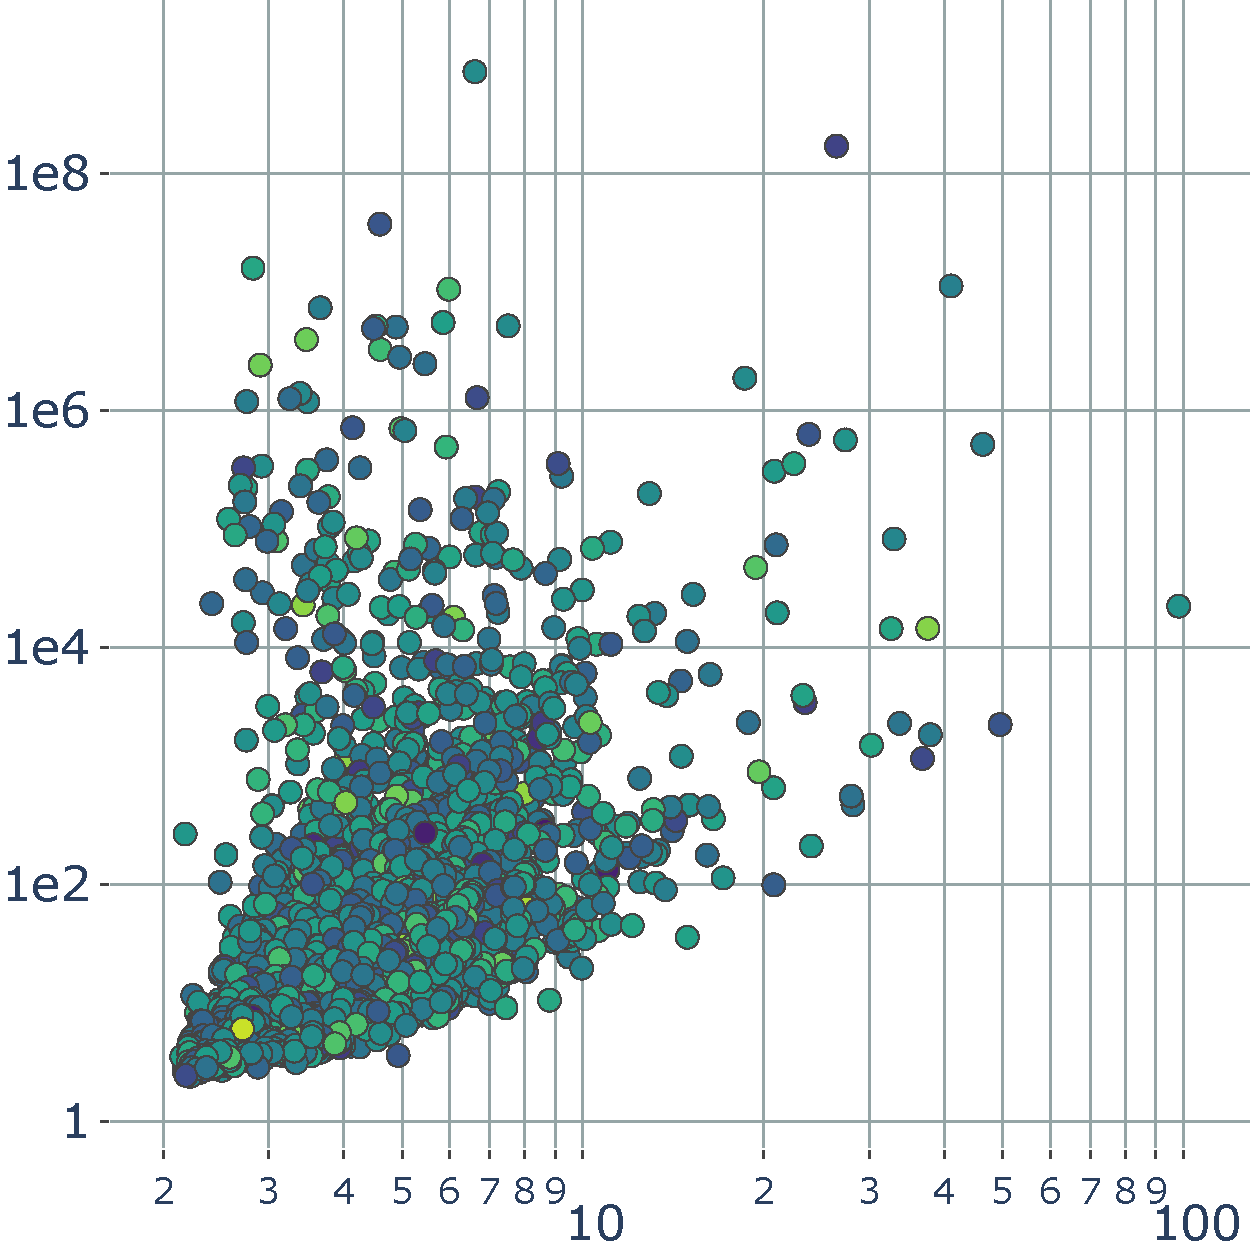
\includegraphics[width=\linewidth]{curve_meshing_in_shell_tex/figs/stats/energy_ABC}}\hfill
    \parbox{.3\linewidth}{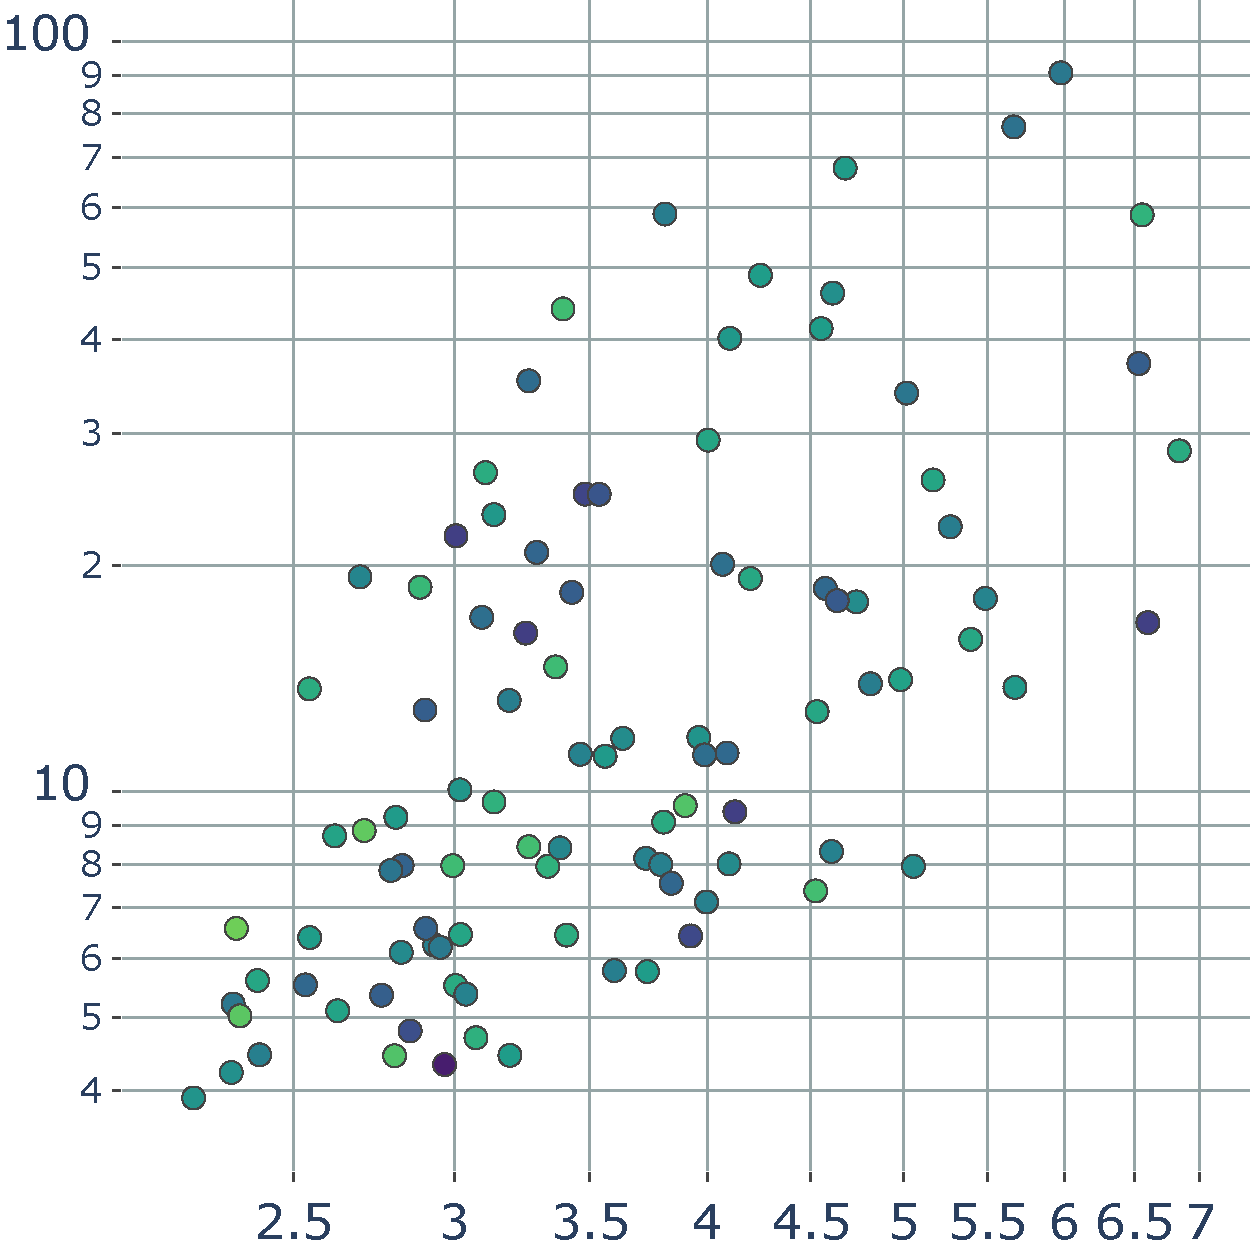
\includegraphics[width=\linewidth]{curve_meshing_in_shell_tex/figs/stats/energy_PoLyCube}}\par
    \scriptsize{Surface Energy}
    \caption{Surface and volume average MIPS energy of the output of our method (the CAD volume energy is truncated at 100, excluding 6 models).}
    \label{bichon:fig:quality}
\end{figure}

The output of our algorithm can be directly used in {the} simulation (Section~\ref{cumin:sec:application}) since we guarantee that the geometric mapping $g$ is positive. To ensure good conditioning and performance of the numerical solver, we measure the MIPS energy~\cite{hormann2000mips,fu2015computing} of our output meshes (Figure~\ref{bichon:fig:quality}). 

\begin{figure}
    \centering
    % \includegraphics{}
    \parbox{0.02\linewidth}{~}\hfill\hfill
    \parbox{.3\linewidth}{\centering Thingi10k}\hfill
    \parbox{.3\linewidth}{\centering ABC}\hfill
    \parbox{.3\linewidth}{\centering CAD}\par
    %
    \parbox{0.02\linewidth}{\centering\rotatebox{90}{\scriptsize{Time(s)}}}\hfill\hfill
    \parbox{.3\linewidth}{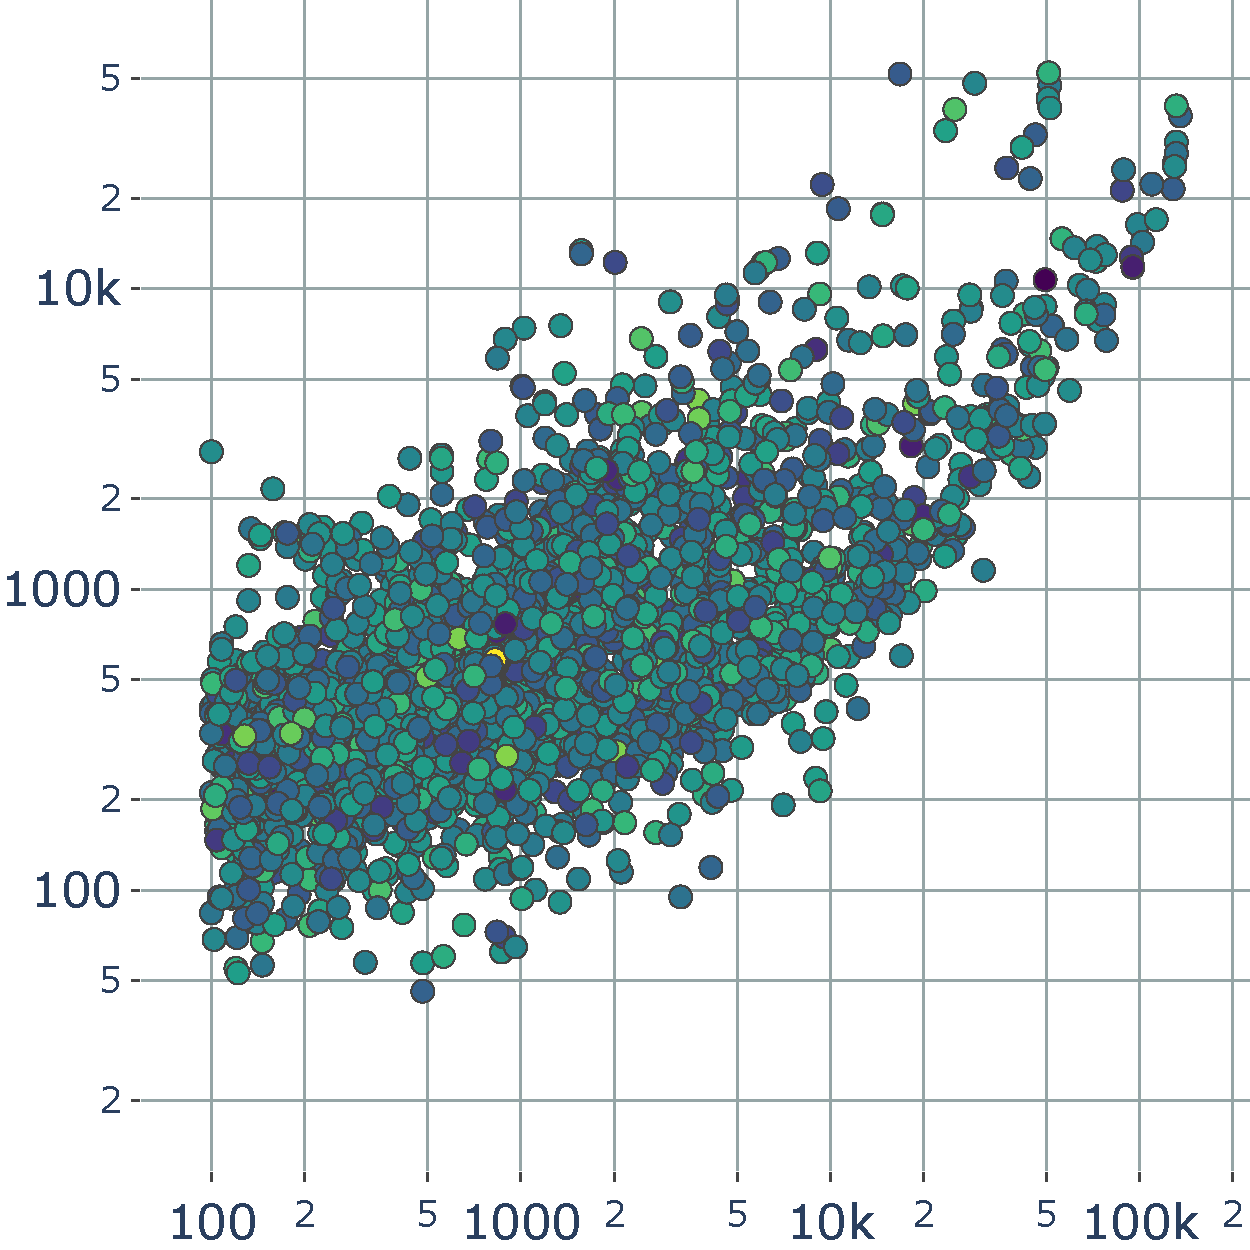
\includegraphics[width=\linewidth]{curve_meshing_in_shell_tex/figs/stats/time_Thingi10k}}\hfill
    \parbox{.3\linewidth}{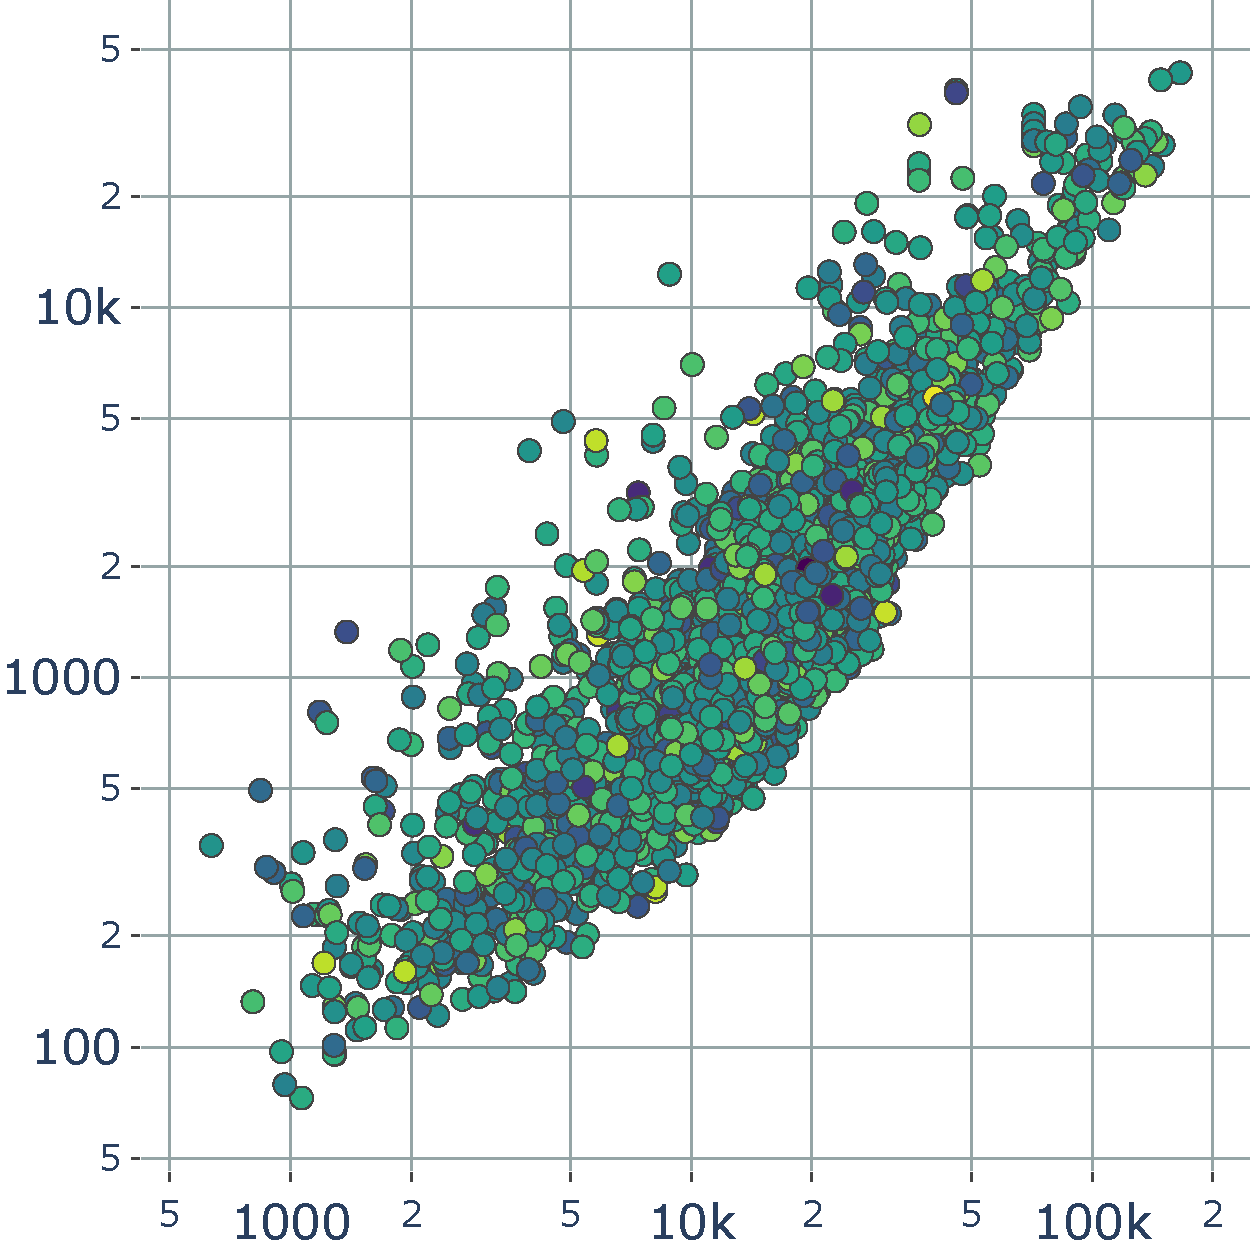
\includegraphics[width=\linewidth]{curve_meshing_in_shell_tex/figs/stats/time_ABC}}\hfill
    \parbox{.3\linewidth}{\includegraphics[width=\linewidth]{curve_meshing_in_shell_tex/figs/stats/time_PoLyCube}}\par
    \scriptsize{Input Vertices}
    \caption{Timing of our algorithm versus the input number of vertices.}
    \label{bichon:fig:timings}
\end{figure}

Figure~\ref{bichon:fig:timings} shows the running time of our method with respect to the number of vertices. The running time of our algorithm is linear with respect to the number of input vertices; it takes around an hour for a model with around 10 thousand vertices.


%%%%%%%%%%%%%%%%%%%%%%%%%%%%%%%%%%%%%%%%%%%%%%%%%%%%%%%%%%%%%%%%%%%
%%%%%%%%%%%%%%%%%%%%%%%%%%%%%%%%%%%%%%%%%%%%%%%%%%%%%%%%%%%%%%%%%%%
\subsection{Comparisons}\label{cumin:sec:comparison}



\paragraph{Curved ODT}
\cite{feng2018curved} is, to the best of our knowledge, the only existing algorithm designed to convert dense triangle meshes into coarse, curved approximations. The input and output are the same as in our algorithm. However, their method does not provide a bijective map between the input and output, does not guarantee to preserve features, has no bound on the distance to the input surface, and does not guarantee that the elements are positive. While our algorithm has been designed to process large collections of data automatically, exposing only a few intuitive options to control the faithfulness to the input, the reference implementation of the curved ODT method provided to us by the authors requires the user to choose multiple \emph{per-model} parameters to achieve good results, and the parameters have a strong effect on the quality and validity of the result (as shown in~\cite[Figure 16]{feng2018curved}). We thus restricted our comparison to only a small selection of models (see additional material) that the authors of \cite{feng2018curved} processed for us.
%
\begin{figure}
    \centering\small
    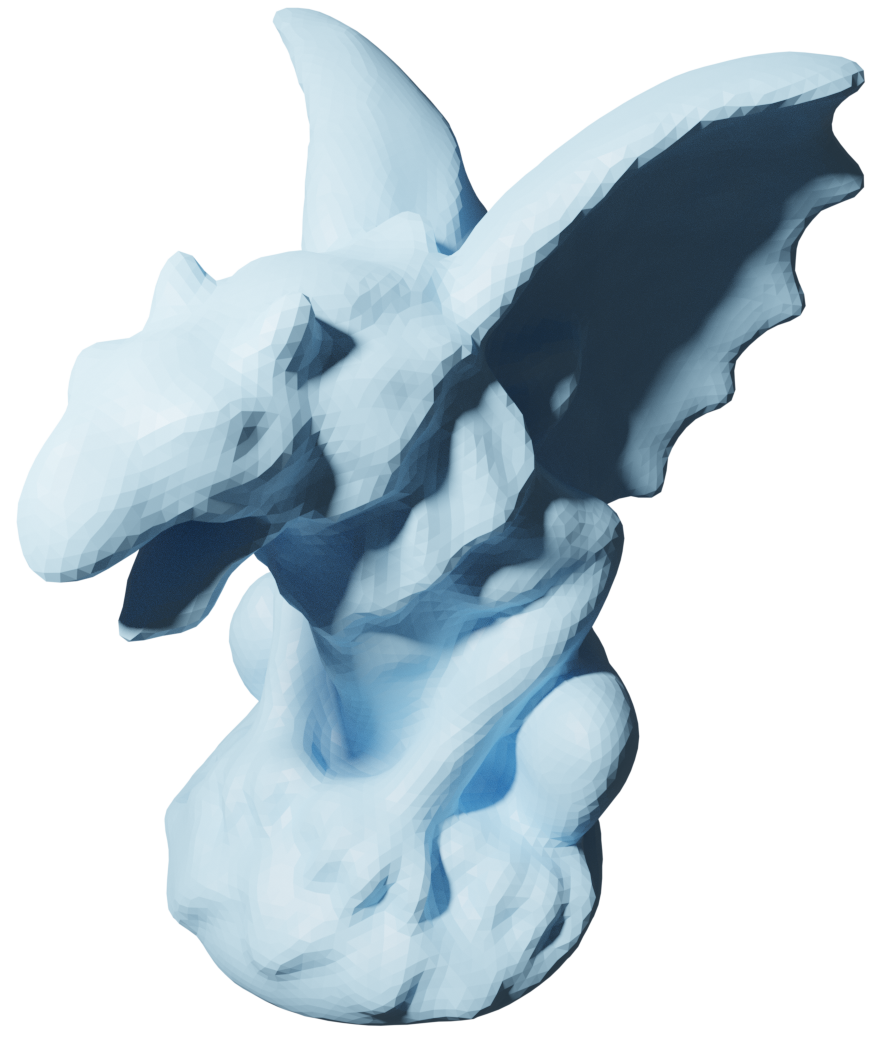
\includegraphics[width=.24\linewidth]{curve_meshing_in_shell_tex/figs/gargo/0001}\hfill
    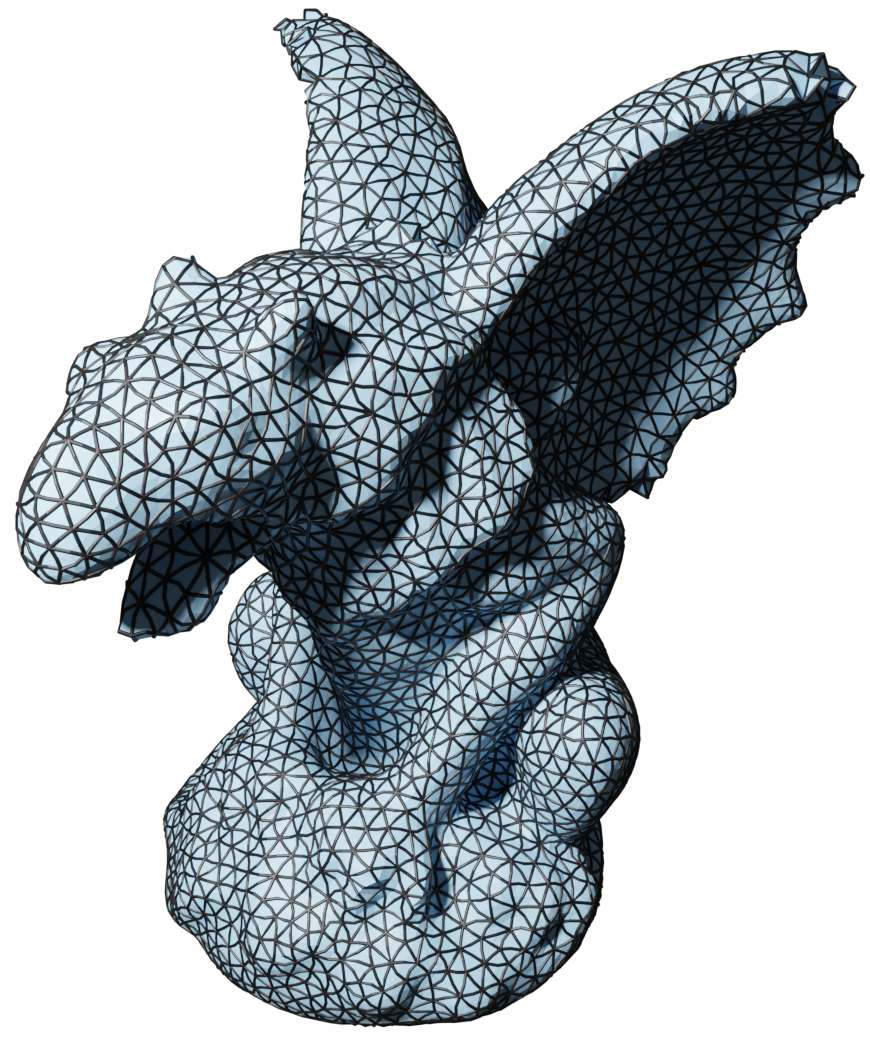
\includegraphics[width=.24\linewidth]{curve_meshing_in_shell_tex/figs/gargo/0002}\hfill
    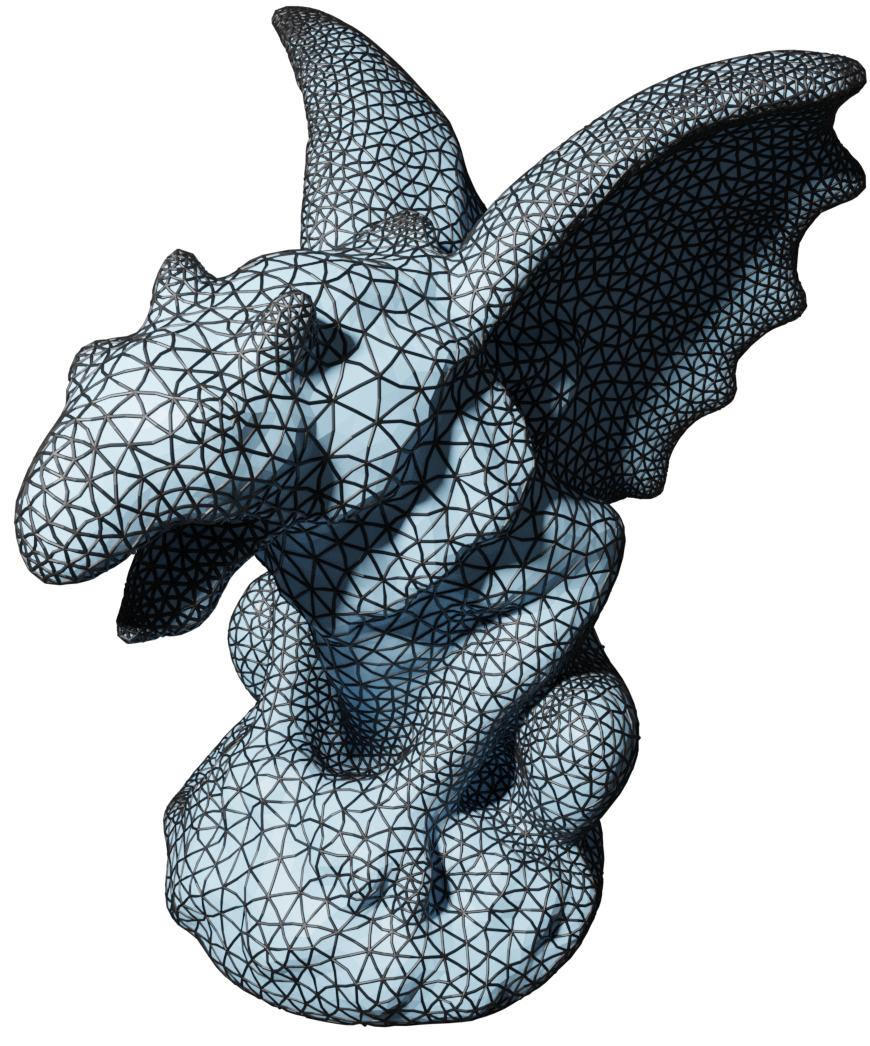
\includegraphics[width=.24\linewidth]{curve_meshing_in_shell_tex/figs/gargo/0003}\hfill
    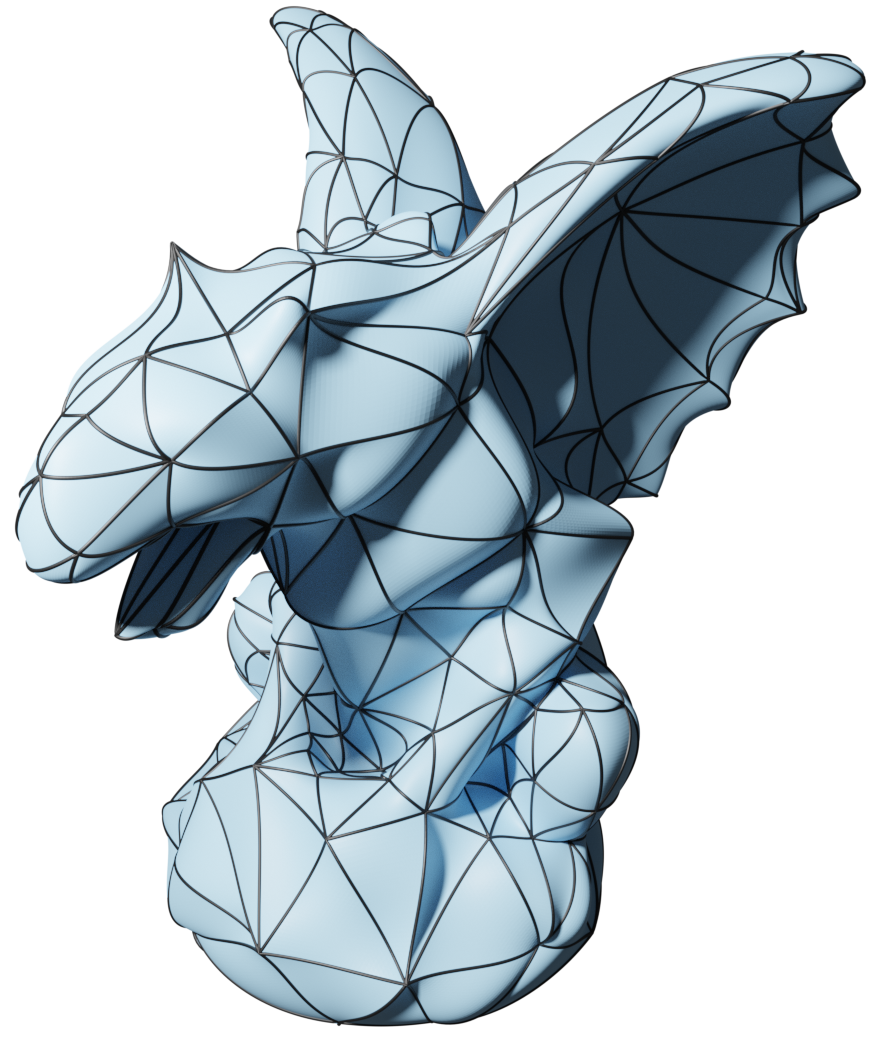
\includegraphics[width=.24\linewidth]{curve_meshing_in_shell_tex/figs/gargo/0004}
    \parbox{.24\linewidth}{\centering Input}\hfill
    \parbox{.24\linewidth}{\centering CODT with uniform\\(46249 elements)}\hfill
    \parbox{.24\linewidth}{\centering CODT with LFS\\(38159 elements)}\hfill
    \parbox{.24\linewidth}{\centering Our\\(2037 elements)}\par
    \caption{Compared with Curved ODT, our method does not rely on setting vertex number and sizing field, and can generate coarse valid results.}
    \label{bichon:fig:cdt}
\end{figure}

From our discussions with the authors, we observed that curved ODT generates a \emph{valid} output when we provide (1) a sufficiently large number of vertices and (2) a good local feature size sizing field (LFS)~\cite{alliez2005variational} to efficiently spend the vertex budget in the regions with more geometrical details.  Figure~\ref{bichon:fig:cdt} shows an example of a model for which \cite{feng2018curved} fails to converge when using a uniform sizing field, while it succeeds when the sizing field is used.

In contrast, our algorithm can be run automatically on {a} large collection of geometrical models, it is guaranteed to have positive Jacobian (up to the use of floating-point predicates, Section~\ref{cumin:sec:conclusion}), it preserves features, it automatically controls the density of the output depending on the desired user-provided distance threshold, and it provides a bijective map between the input mesh the boundary of the curved surface. For the model in Figure \ref{bichon:fig:cdt}, our result contains 2037 elements, 18 times less than the curved ODT algorithm. %We note that the LFSSF is brittle and the authors were unable to generate it for complex models with features (see additional material), thus their algorithm fails.


\begin{figure}
    \centering\small
    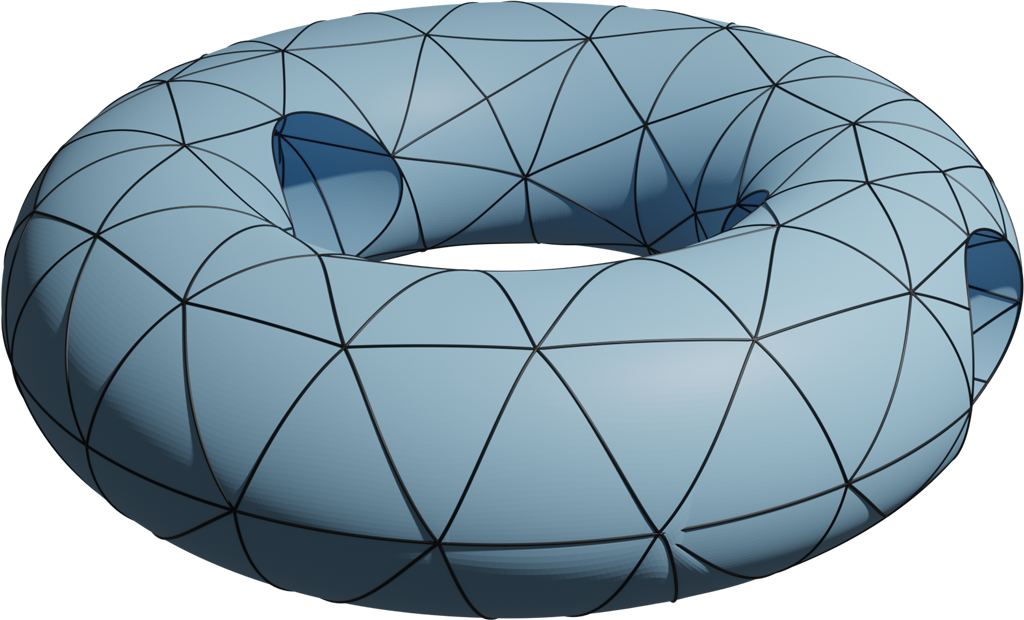
\includegraphics[width=0.32\linewidth]{curve_meshing_in_shell_tex/figs/gmsh/not-bij}\hfill
    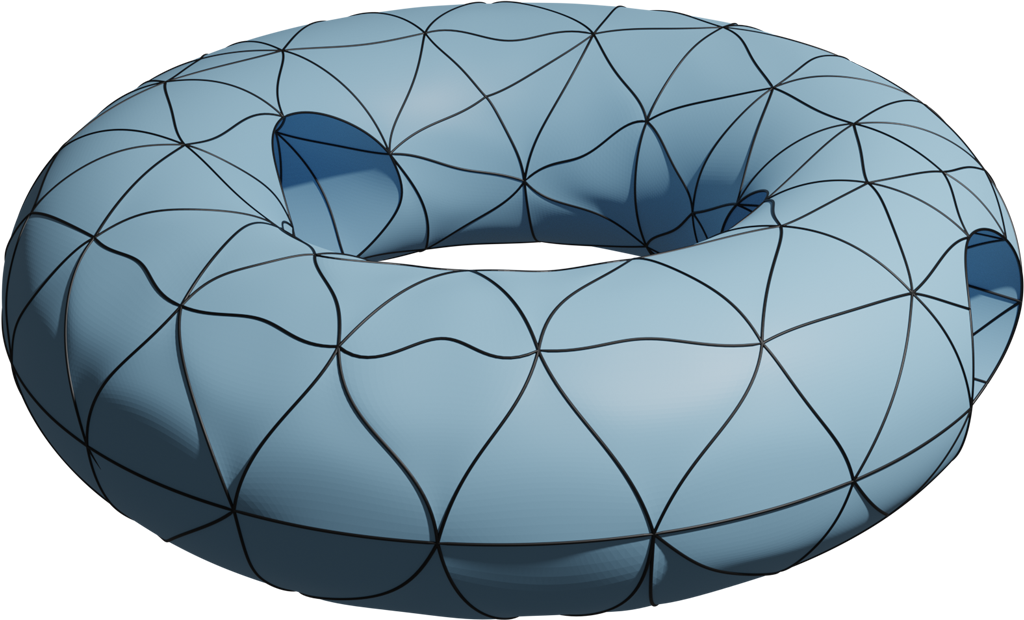
\includegraphics[width=0.32\linewidth]{curve_meshing_in_shell_tex/figs/gmsh/bij}\hfill
    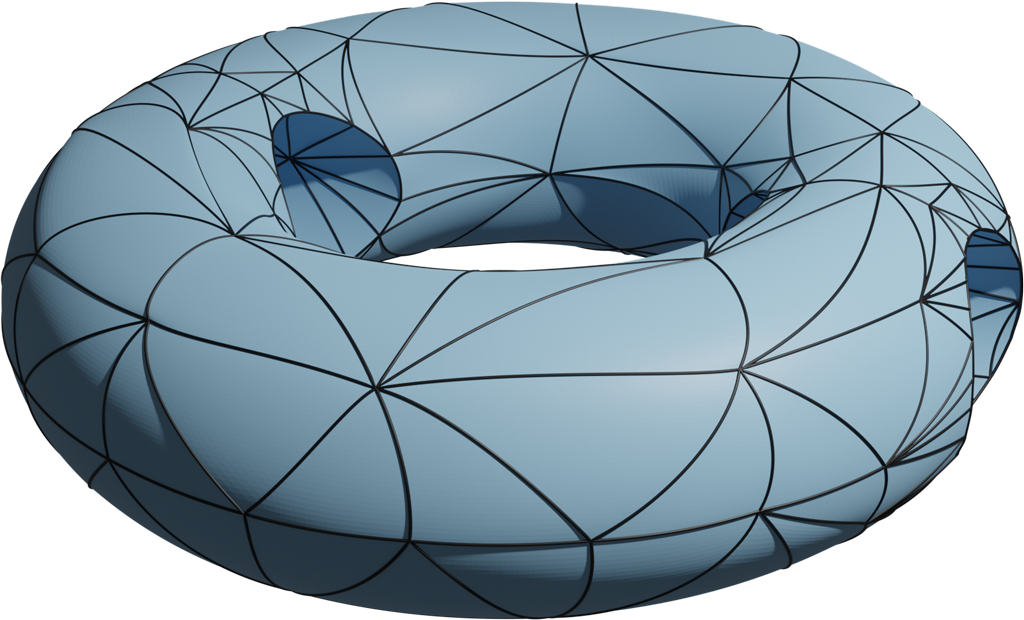
\includegraphics[width=0.32\linewidth]{curve_meshing_in_shell_tex/figs/gmsh/torus}
     \parbox{.32\linewidth}{\centering Gmsh Fixed Surface}\hfill
    \parbox{.32\linewidth}{\centering Gmsh Free Surface}\hfill
    \parbox{.32\linewidth}{\centering Ours}\par
    \caption{Example of a BRep meshed with Gmsh where the optimization fails to untangle elements when fixing the surface. By allowing the surface to be modified, the mesh becomes ``wiggly''. Our method successfully generate a positive curved mesh.}
    \label{bichon:fig:gmsh-flipped}
\end{figure}


\begin{figure}
    \centering\small
    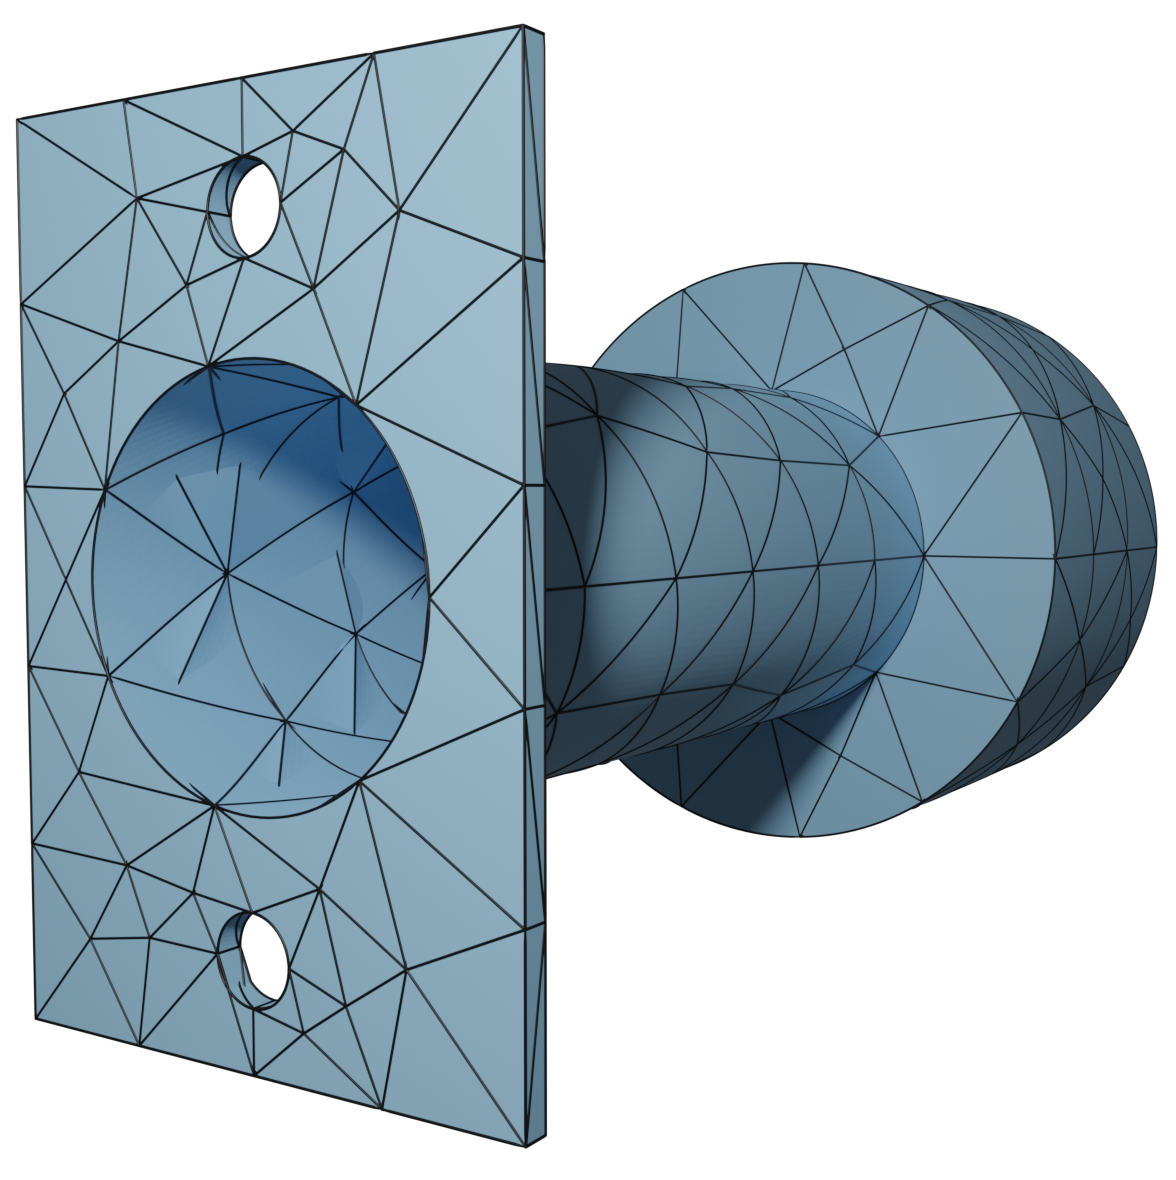
\includegraphics[width=.32\linewidth]{curve_meshing_in_shell_tex/figs/gmsh/step/0001}\hfill
    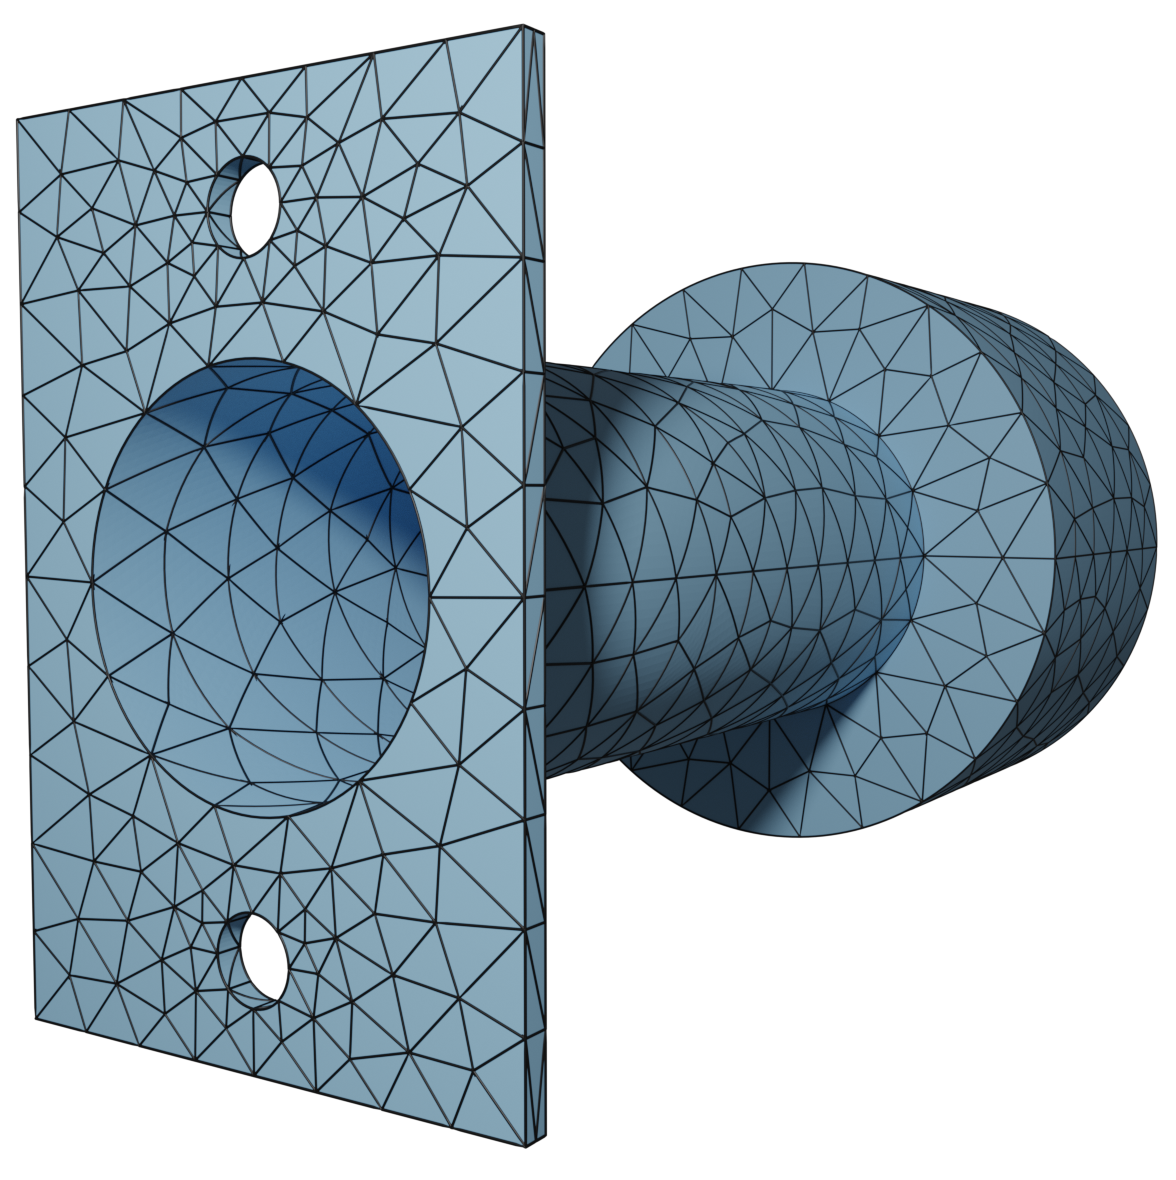
\includegraphics[width=.32\linewidth]{curve_meshing_in_shell_tex/figs/gmsh/step/0002}\hfill
    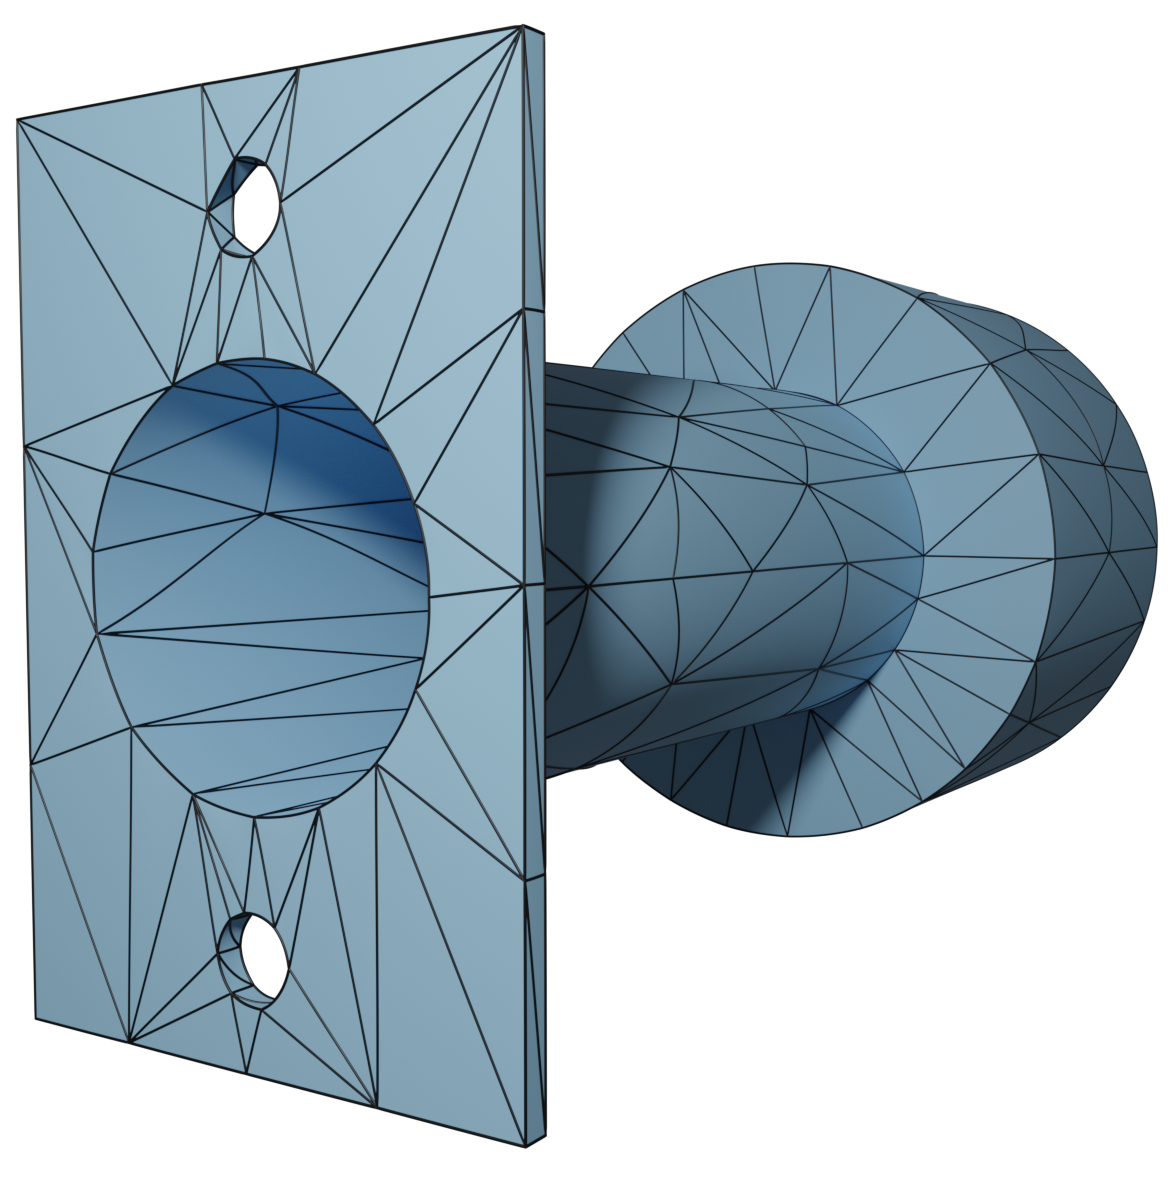
\includegraphics[width=.32\linewidth]{curve_meshing_in_shell_tex/figs/gmsh/step/0003}\par
    \parbox{.32\linewidth}{\centering Coarse Gmsh}\hfill
    \parbox{.32\linewidth}{\centering Dense Gmsh}\hfill
    \parbox{.32\linewidth}{\centering Ours}\par
    \caption{Example of a STEP file meshed with Gmsh where, due to the low mesh density, the tetrahedralization is not positive. Gmsh manages to generate a positive mesh by using a denser initial  tessellation. Since our method starts from a dense mesh and coarsen it, it can successfully resolve the geometry.}
    \label{bichon:fig:closed-holes}
\end{figure}
\paragraph{Gmsh}
\cite{Geuzaine:2009:gmsh} can only generate curved meshes from boundary representation (BRep), that is the input is not exactly the same as ours. To compare both algorithms, we start from the BRep and we generate a dense \emph{linear} mesh that we use for our input. The Gmsh algorithm {first} constructs a curved mesh by fitting the high-order nodes to the BRep (possibly inverting elements) then performs mesh optimization to untangle them~\cite{remacle2013robust}; thus has no guarantee to generate positive meshes while preserving the surface (Figure~\ref{bichon:fig:gmsh-flipped}, left). Additionally, Gmsh algorithm cannot control the distance from the input when the untangling allows the surface to move, and thus the surface is ``wiggly'' and denser than our result (Figure~\ref{bichon:fig:gmsh-flipped}, center). We also observed that if the initial surface mesh is not dense enough, Gmsh closes holes and cannot generate a valid tetrahedral mesh (Figure~\ref{bichon:fig:closed-holes}).


%%%%%%%%%%%%%%%%%%%%%%%%%%%%%%%%%%%%%%%%%%%%%%%%%%%%%%%%%%%%%%%%%%%
%%%%%%%%%%%%%%%%%%%%%%%%%%%%%%%%%%%%%%%%%%%%%%%%%%%%%%%%%%%%%%%%%%%
\subsection{Flexibility}

\begin{figure}
    \centering\small
    %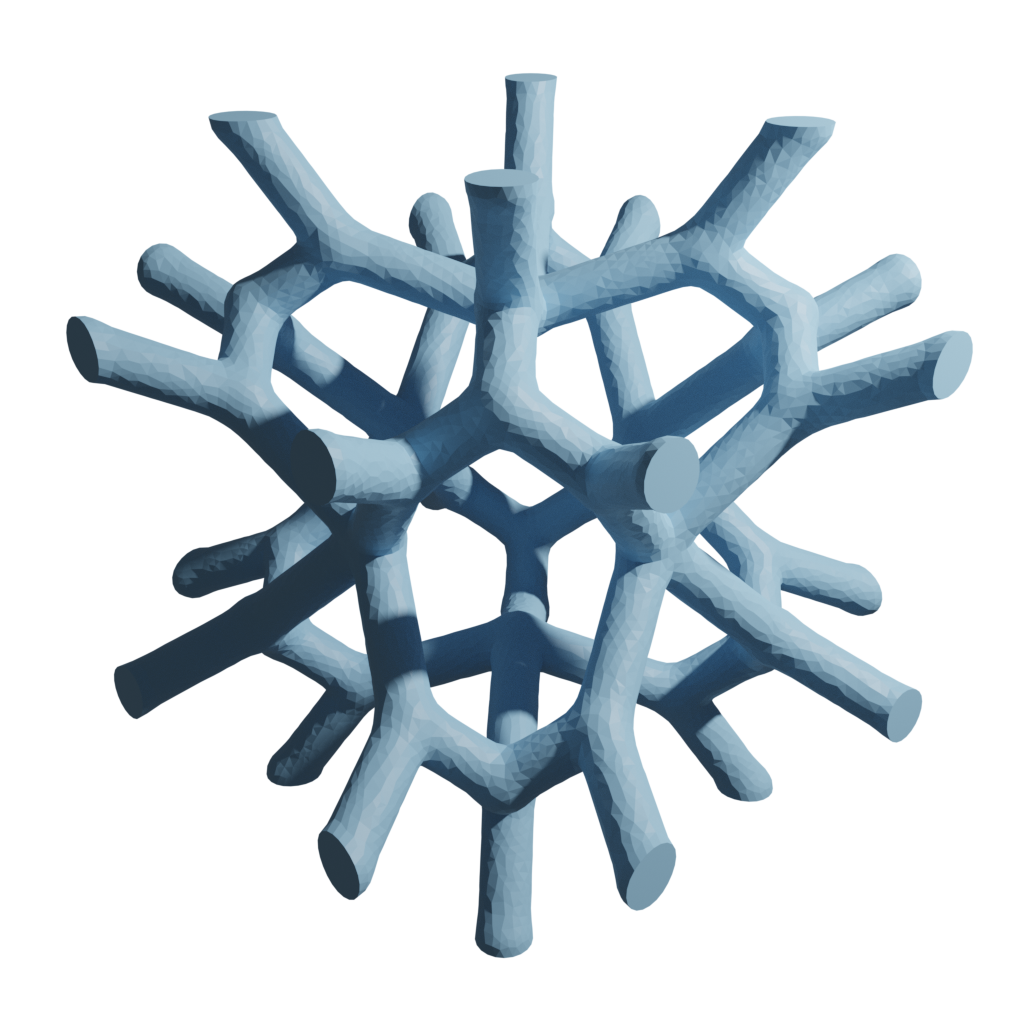
\includegraphics[width=0.45\linewidth]{curve_meshing_in_shell_tex/figs/micro/0001}\hfill
    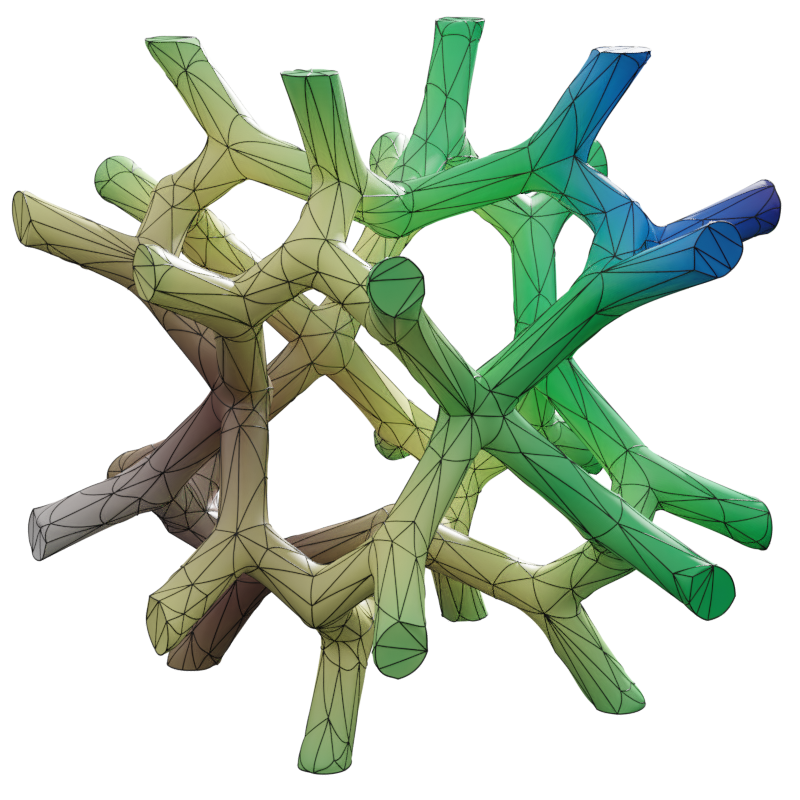
\includegraphics[width=0.49\linewidth]{curve_meshing_in_shell_tex/figs/micro/color}\hfill
    %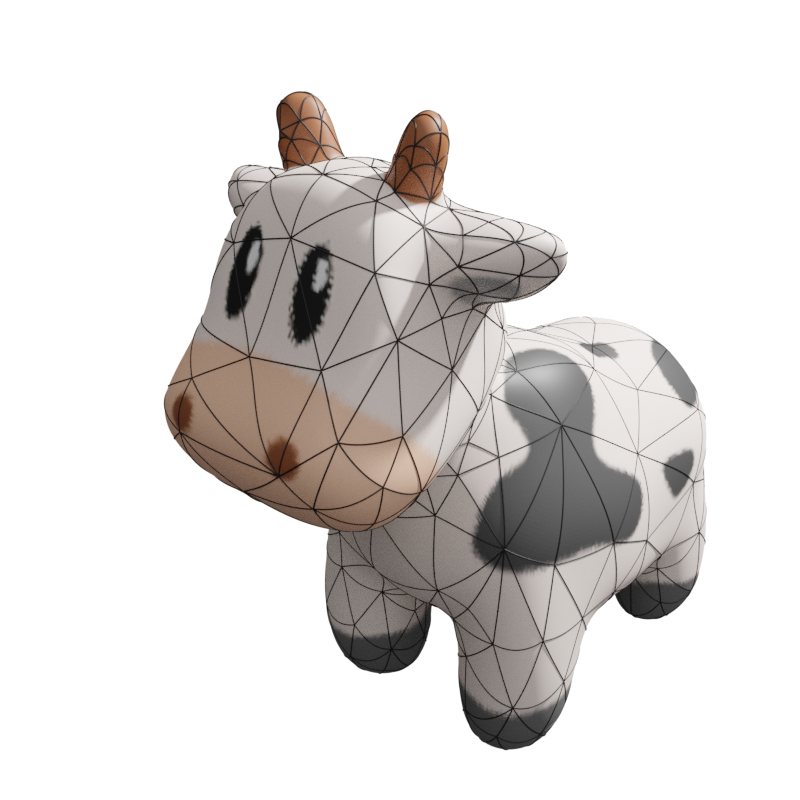
\includegraphics[width=0.45\linewidth]{curve_meshing_in_shell_tex/figs/spot.png}\hfill
    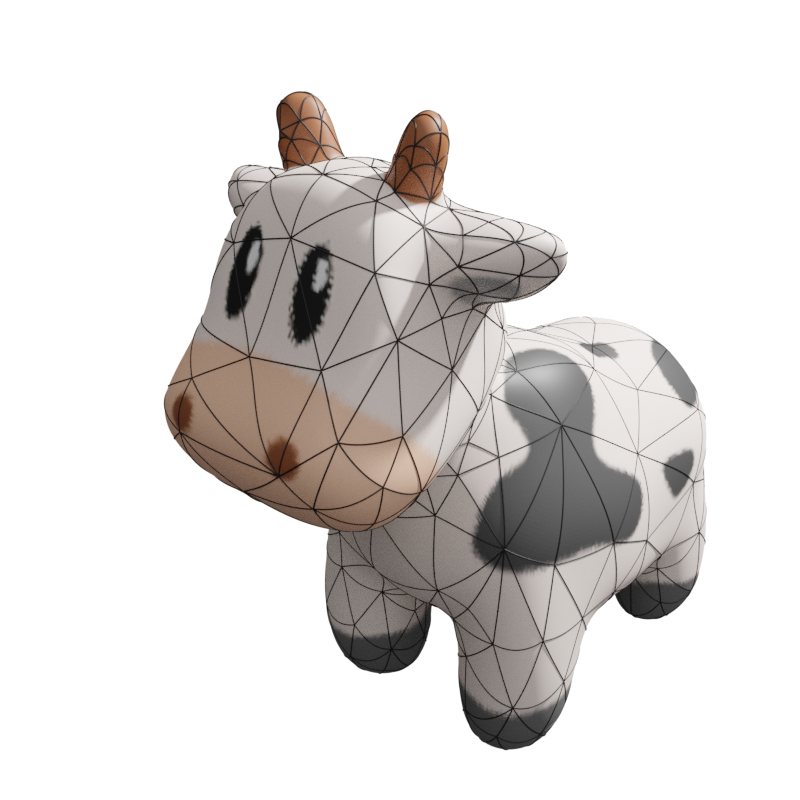
\includegraphics[width=0.49\linewidth]{curve_meshing_in_shell_tex/figs/spot.png}\par
    \parbox{.49\linewidth}{\centering Implicit microstructure}\hfill
    \parbox{.49\linewidth}{\centering {subdivision} surface}
    \caption{Our algorithm processes triangle meshes that can be extracted from different formats: an implicit  microstructure geometry from \cite{tozoni2020low} or a subdivision surface from  \cite{crane2013conformal}. The bijective map preserved on the surface allows taking advantage of the plethora of surface algorithms including polyhedral geodesic computation \cite{mitchell1987discrete} and texture mapping.}
    \label{bichon:fig:flex}
\end{figure}

Since the input to our method is a triangle mesh, our method naturally supports a variety of input that can be easily converted into triangle meshes. For instance, $\M$ can be {generated from} marching an implicit surface or Catmull-Clark subdivision of a hand-made quad mesh (Figure~\ref{bichon:fig:flex}). The bijective map $\phi^k$ {is used}, for instance, to transfer the geodesic distance field or color information from the input triangle mesh to the coarse curved mesh.


%%%%%%%%%%%%%%%%%%%%%%%%%%%%%%%%%%%%%%%%%%%%%%%%%%%%%%%%%%%%%%%%%%%
%%%%%%%%%%%%%%%%%%%%%%%%%%%%%%%%%%%%%%%%%%%%%%%%%%%%%%%%%%%%%%%%%%%
\subsection{Applications}\label{cumin:sec:application}


\begin{figure}
    \centering
    % \includegraphics{}
    \parbox{0.01\linewidth}{~}\hfill\hfill
    \parbox{.3\linewidth}{\centering Thingi10k}\hfill
    \parbox{.3\linewidth}{\centering ABC}\hfill
    \parbox{.3\linewidth}{\centering CAD}\par
    %
    \parbox{0.01\linewidth}{\centering\rotatebox{90}{\scriptsize{$L^2$ error}}}\hfill\hfill
    \parbox{.3\linewidth}{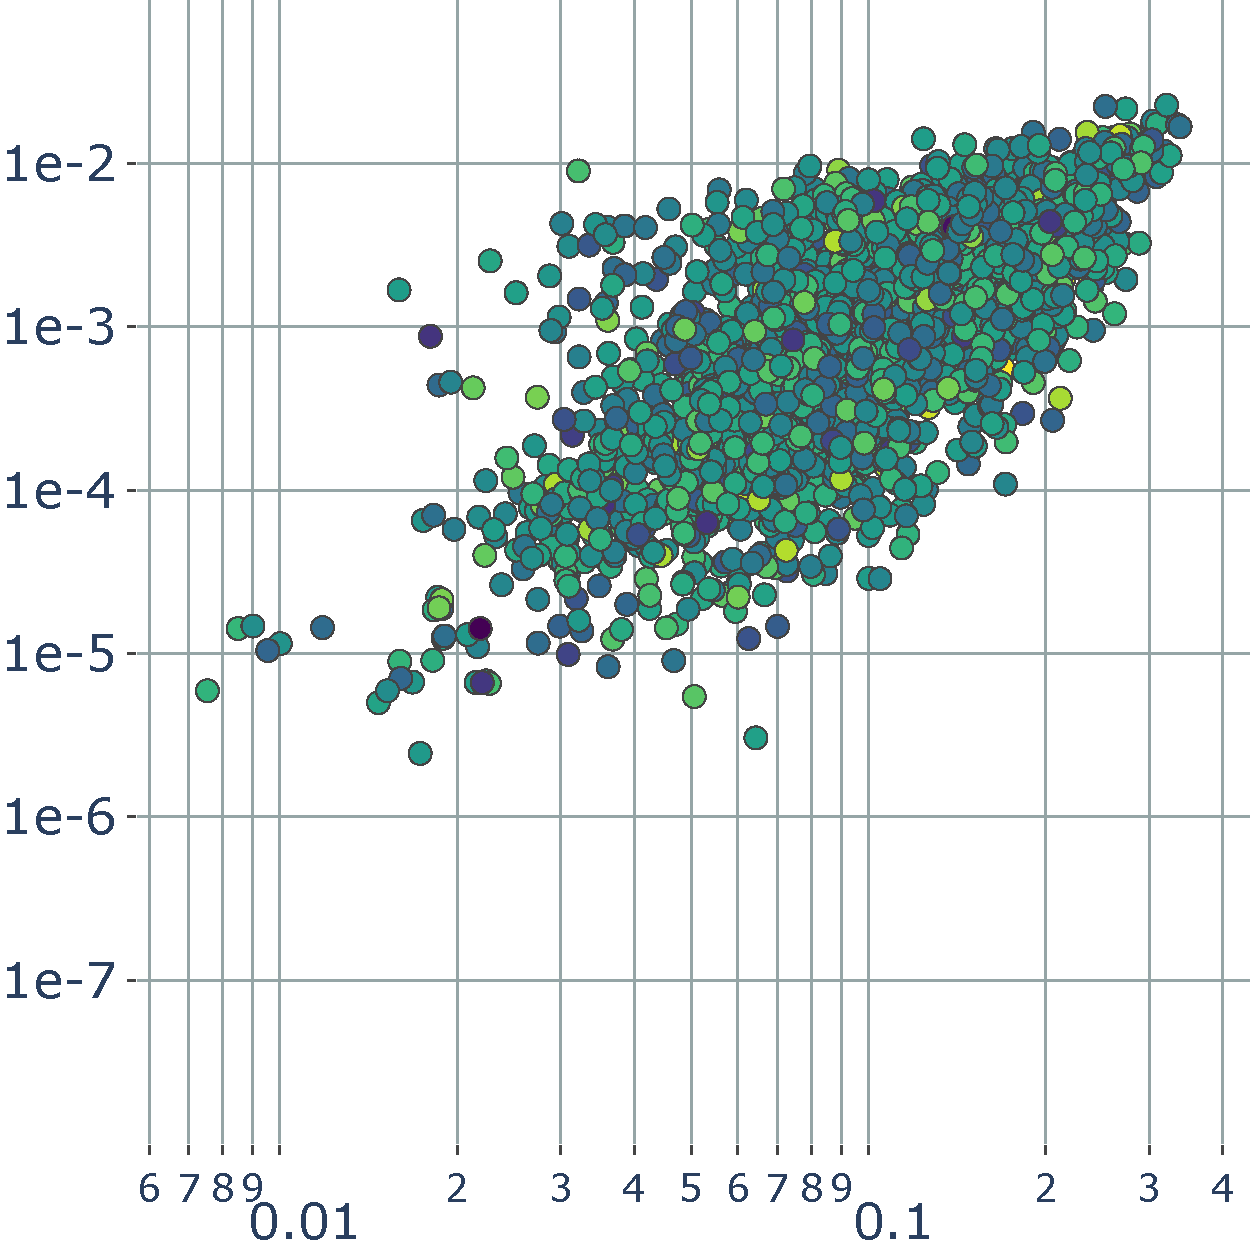
\includegraphics[width=\linewidth]{curve_meshing_in_shell_tex/figs/stats/error_Thingi10k}}\hfill
    \parbox{.3\linewidth}{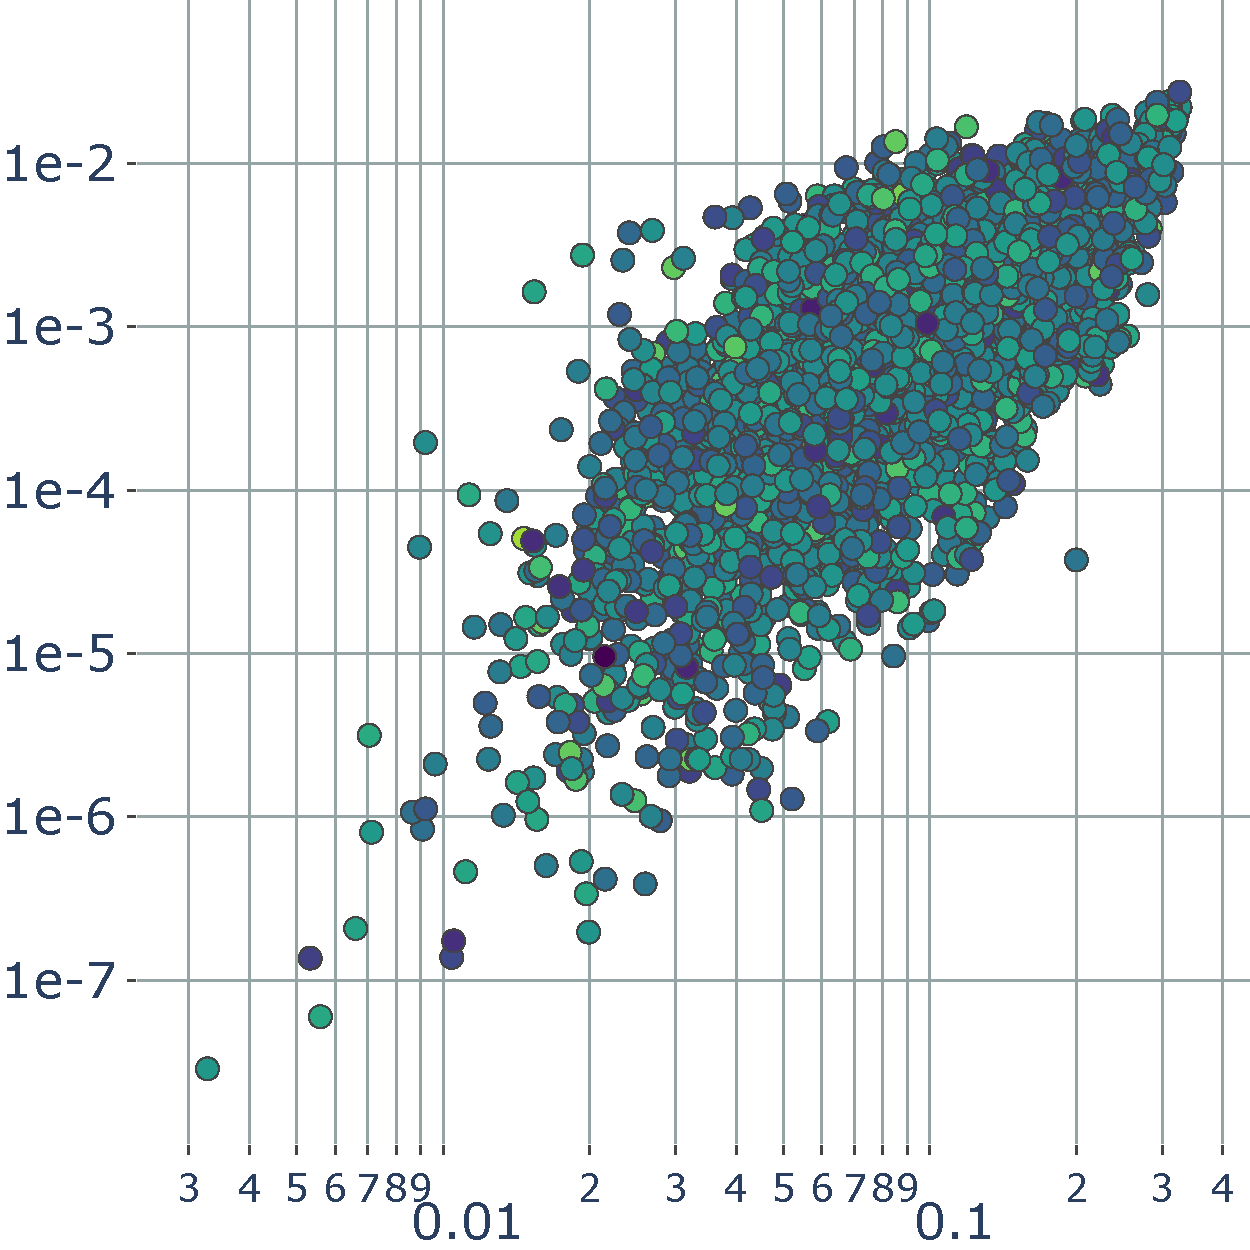
\includegraphics[width=\linewidth]{curve_meshing_in_shell_tex/figs/stats/error_ABC}}\hfill
    \parbox{.3\linewidth}{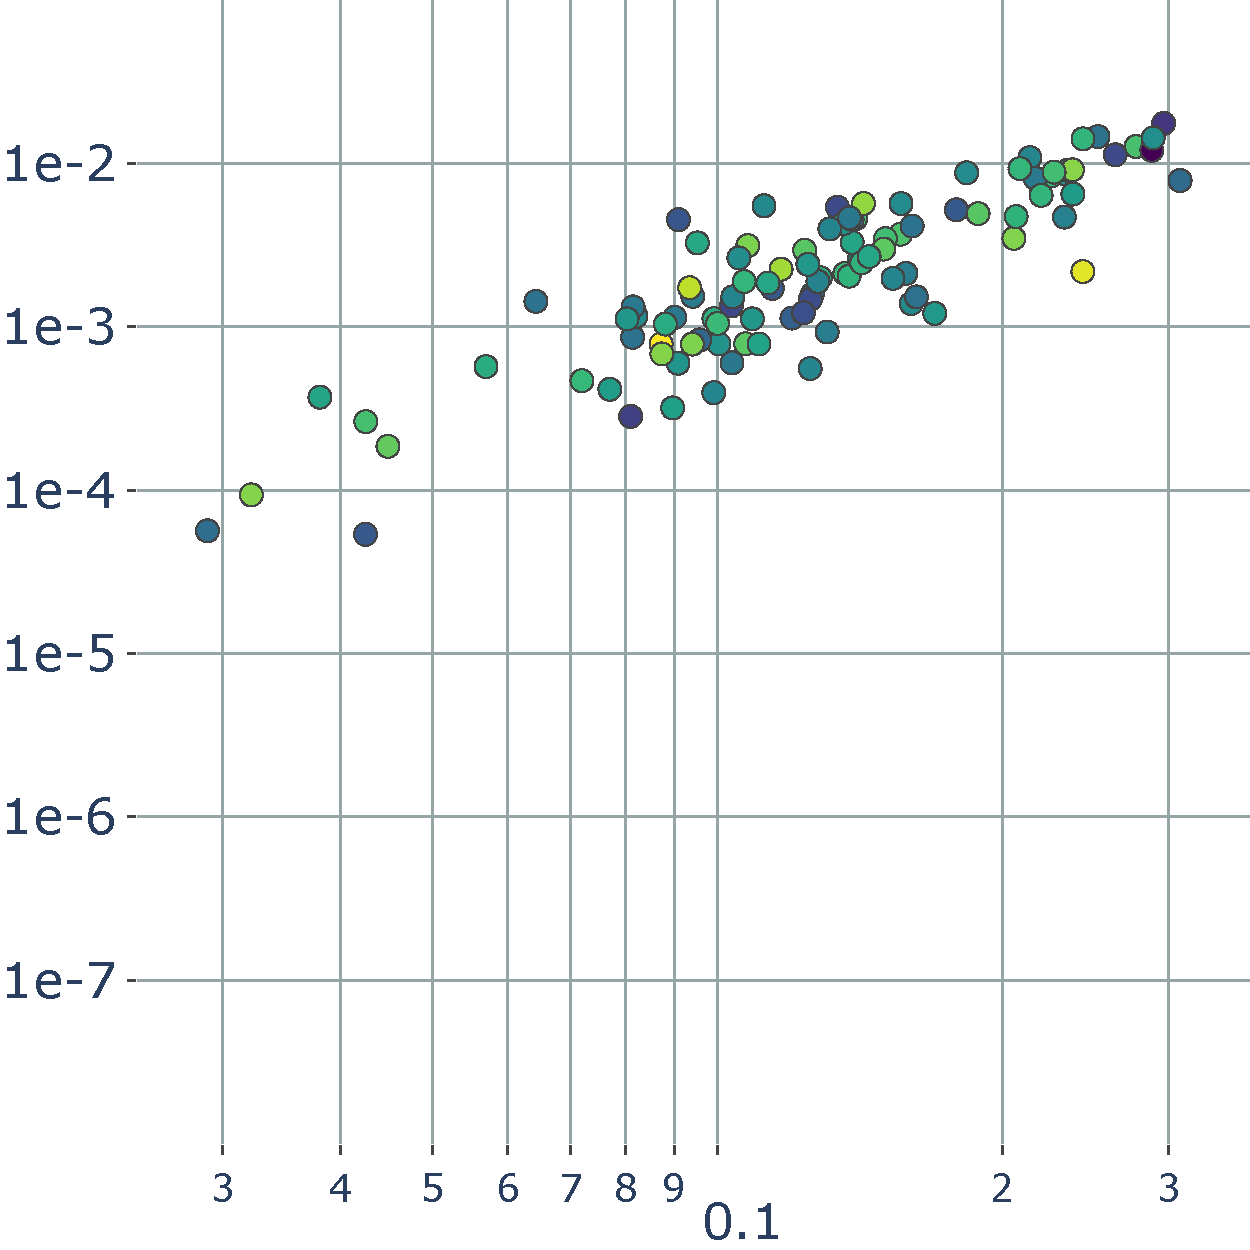
\includegraphics[width=\linewidth]{curve_meshing_in_shell_tex/figs/stats/error_PolyCube}}\par
    \scriptsize{Average Edge Length}
    \caption{$L^2$ error of the solution of the Poisson equation with respect to model size on our three datasets.}
    \label{bichon:fig:large-scale-poisson}
\end{figure}

\paragraph{Large Scale Poisson}
To show that our meshes are ready for simulation, we solve for Poisson equation
\[
\Delta u  = f,\quad
u|_{\partial \Omega} = g,
\]
where $\Omega$ is the domain (i.e., the mesh), $f$ is the right-hand side, and $g$ are the Dirichlet boundary conditions. To simplify the setup and the error measurements, we use fabricated solutions~\cite{SALARI:2000:CVB}. That is, we choose the function $u_\text{exact}$ to be {%\scriptsize
\begin{align*}
u_\text{exact}&(x_1,x_2,x_3) =
\\&3/4\,{ e}^{-((9x_1-2)^2+(9x_2-2)^2+(9x_3-2)^2)/4}+
3/4\,{ e}^{-(9x_1+1)^2/49-(9x_2+1)/10-(9x_3+1)/10} \\
%
&+1/2\,{ e}^{-((9x_1-7)^2+(9x_2-3)^2+(9x_3-5)^2)/4}-
1/5\,{ e}^{-(9x_1-4)^2-(9x_2-7)^2-(9x_3-5)^2},
\end{align*}}
then we plug it in the equation to obtain $f$ ($g$ is simply $u_\text{exact}$). Figure~\ref{bichon:fig:large-scale-poisson} shows the $L^2$ error (average) distribution across our three datasets using our quartic meshes with quadratic approximation of $u$ (i.e., we use superparametric elements).


\begin{figure}
    \centering\small
    % 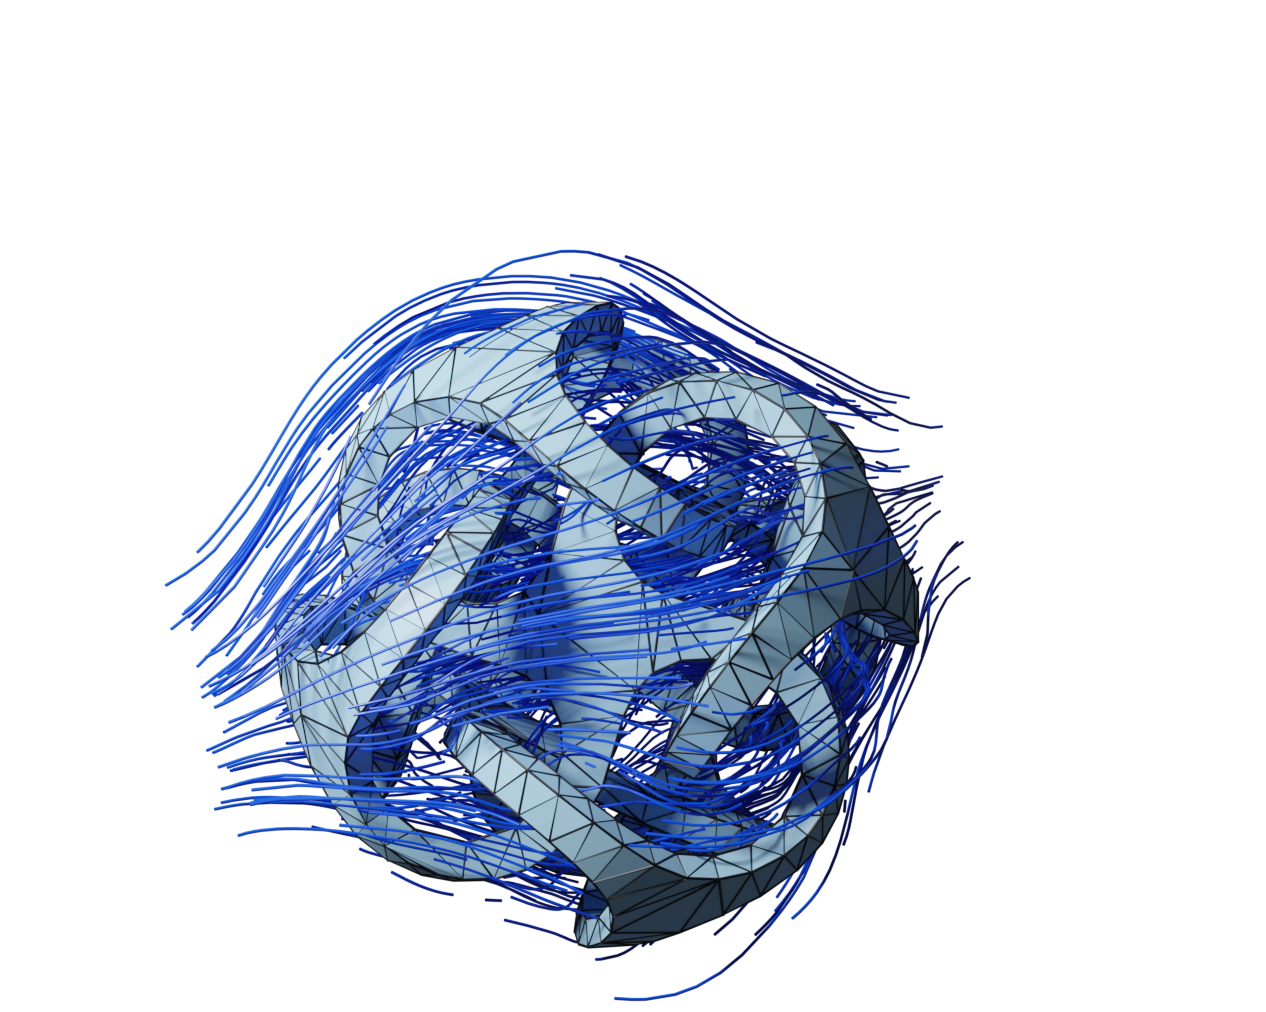
\includegraphics[width=.32\linewidth]{curve_meshing_in_shell_tex/figs/fluid/0001}\hfill
    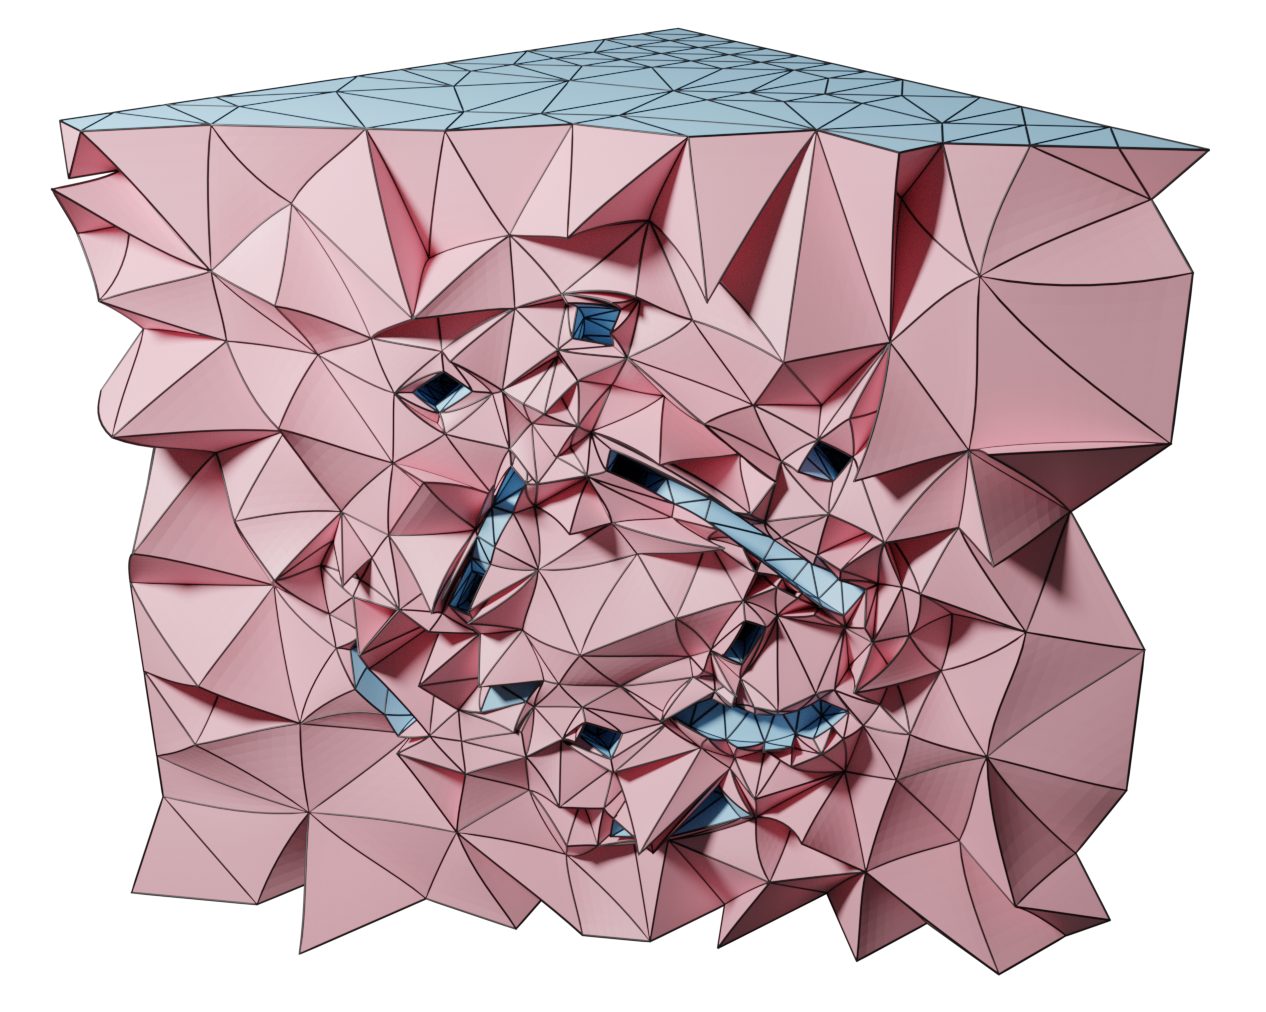
\includegraphics[width=.45\linewidth]{curve_meshing_in_shell_tex/figs/fluid/0003}\hfill
    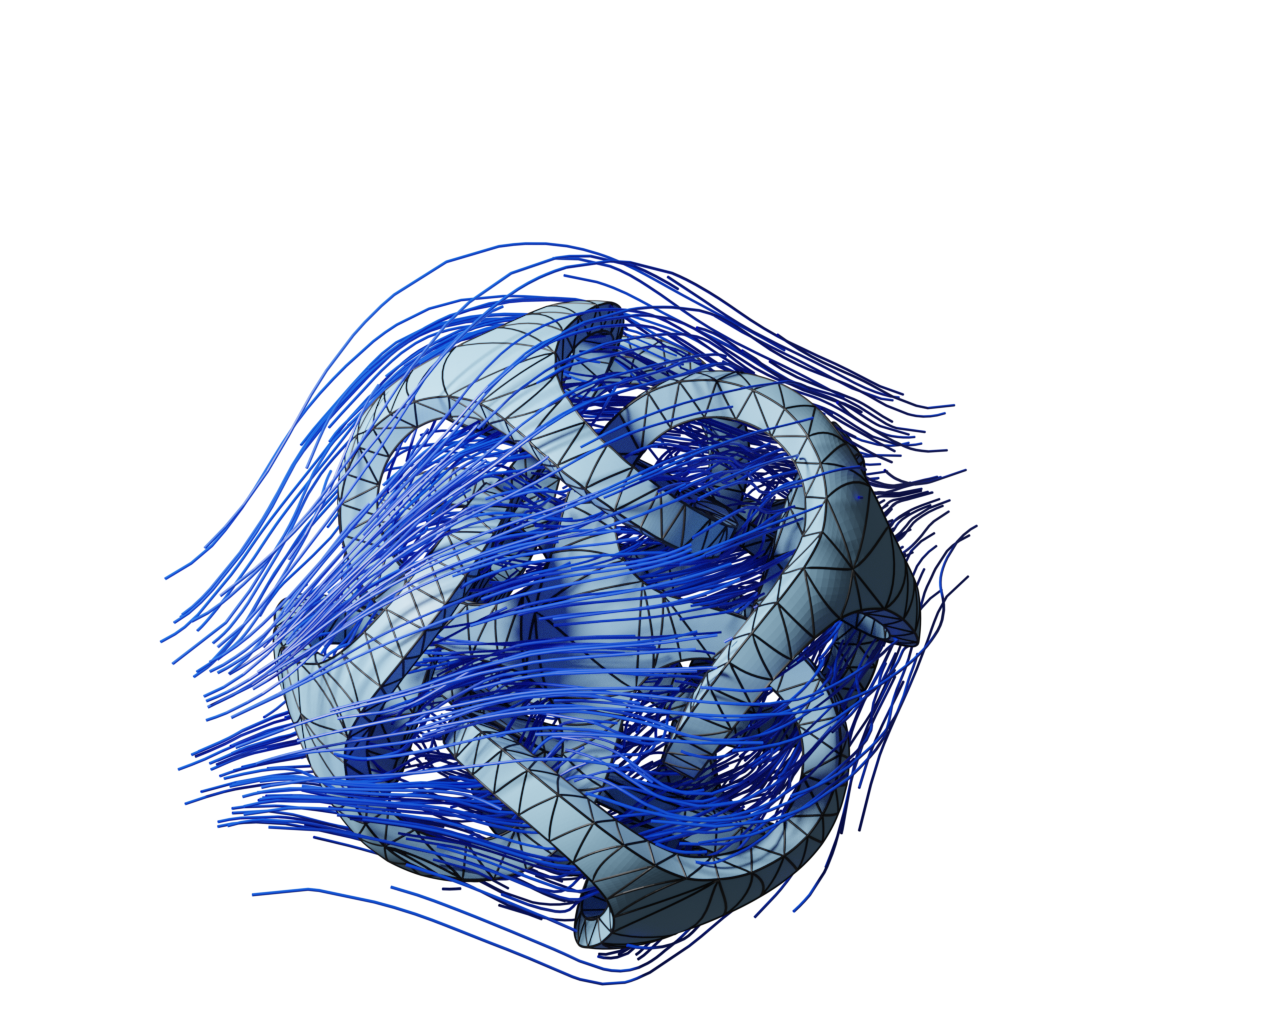
\includegraphics[width=.53\linewidth]{curve_meshing_in_shell_tex/figs/fluid/0002}\hfill
    % 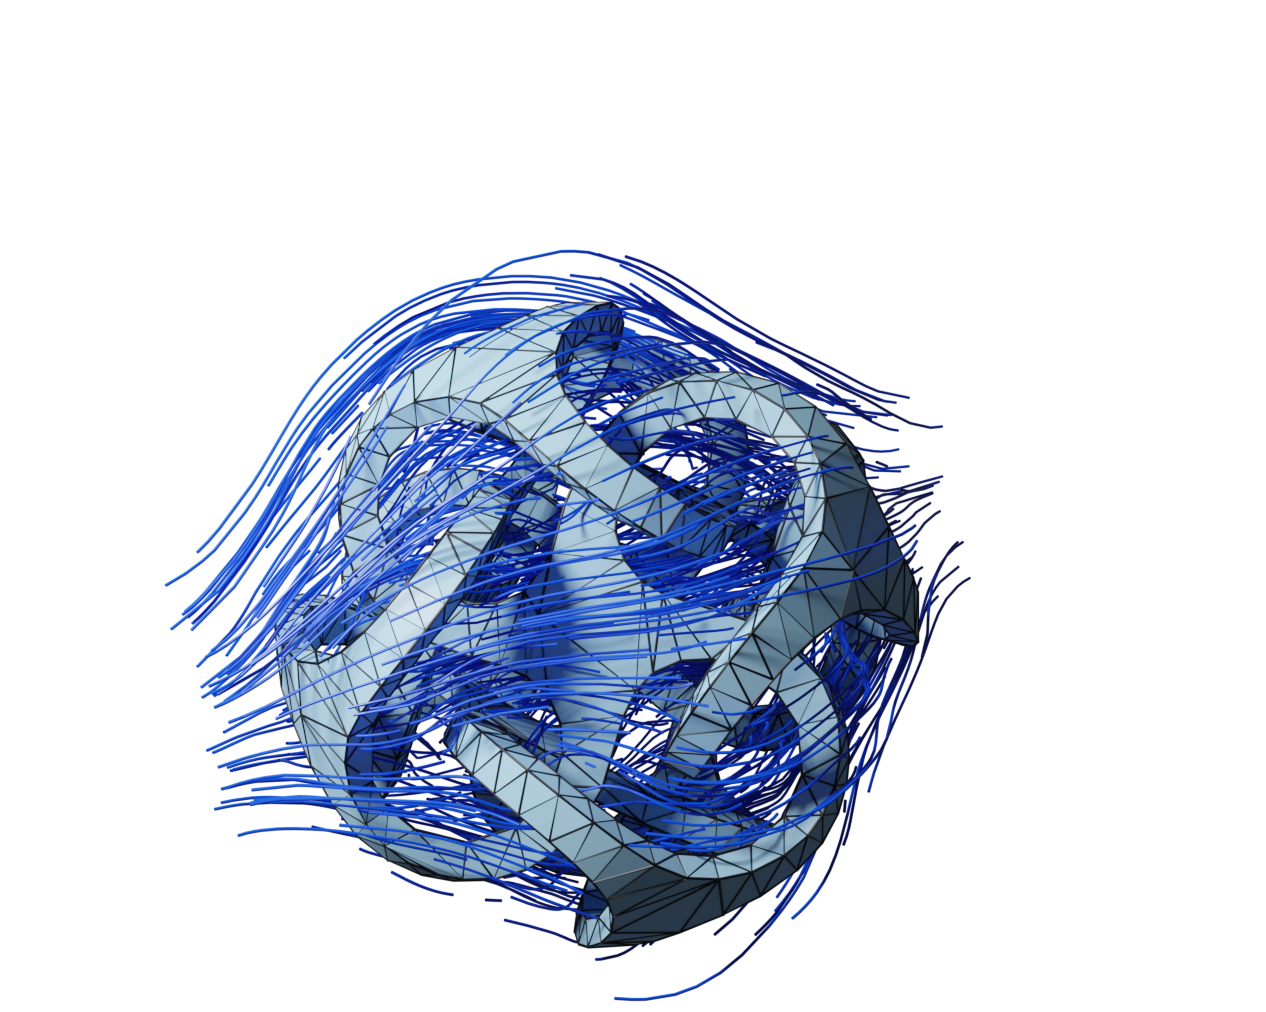
\includegraphics[width=.32\linewidth]{curve_meshing_in_shell_tex/figs/fluid/0001}\par
    \parbox{.45\linewidth}{\centering Tetrahedral mesh}\hfill
    \parbox{.53\linewidth}{\centering Curved simulation}\hfill
    % \parbox{.32\linewidth}{\centering Linear simulation}
    \caption{By meshing the region between a box and a complicated obstacle, we are able to perform non-linear fluid simulation on our curved mesh.}
    \label{bichon:fig:ns}
\end{figure}
\paragraph{High Accuracy Fluids}
Our curved meshes can be directly used to solve different partial differential equations (PDEs). For instance, by meshing the part outside the top shell and discarding the rest, we can generate a curved background mesh for the Navier-Stokes equation (Figure~\ref{bichon:fig:ns}). 

%took 5.01566s

% \begin{figure}
%     \centering
%     % \includegraphics{}
%     \TODO{do me}
%     \caption{Example of using a curved mesh as animation proxy.}
%     \label{bichon:fig:anim}
% \end{figure}
\paragraph{Fast Animation}
Our coarse curved meshes can be {used} as animation proxies as in~\cite{mezger2007finite,Suwelack2013}. We first compute an as-coarse-as-possible curved mesh (i.e., we set $\varepsilon$ to infinity). Then we apply the boundary condition to simulate an elastic distortion of the curved mesh using linear elements. Finally, we use our bijective map $\varphi^4$ to map the displacement back to the input high-detailed surface mesh (Figure~\ref{bichon:fig:teaser}). The results are almost indistinguishable {to} a classical pipeline (i.e., mesh the input mesh), but the runtime is 400 times faster (8s versus over 50 minutes). 



% \paragraph{Tessellation Shading}
% \TODO{probably skip, if we do, we can rename the section}
% rendering example, as coarse as possible, high error is ok, simplifying seams

%\subsection{Rendering}
% \subsection{Reverse Engineering}
% Triangle mesh to CAD.
% \subsection{Simulation efficiency?}